
\chapter{A modular synthesis engine}
\label{sec:04-graph}

\epigraph{We can now see that the whole becomes not merely more, but
  very different from the sum of its parts.}{\emph{More is Different:
  Broken Symmetry and the Nature of the Hierarchical Structure of
  Science}\\\textsc{Philip Warren Anderson}}

\section{Analysis}

In the previous chapter we built a system for sound representation,
processing, and interfacing. In such system, interactions
between different processing elements is hard-coded in the control
flow of the program itself and the relations among the statically
parametrised types that intervene.

As described by requirements \ref{req:iter2-begin} to
\ref{req:iter2-end}, we shall develop a system where the basic DSP
units can be composed orthogonally and hierarchically to build complex
devices \emph{at runtime}. With the applications built on top of our
framework being targeted at live performances, it should be
particularly dynamic.

\subsection{An abstract model of a modular synthesiser}

\index{modular synthesiser}In a modular synthesiser, the sound
generation is made by interconnecting basic processing units. Each of
them might generate sound, filter it, and can have a varying number of
inputs and outputs of different kinds. Because a \index{module (DSP)}
module can apply virtually any mathematical function to its inputs; we
can realise any synthesis technique --- i.e. additive, subtractive,
FM/PM --- by just wiring the available modules in an appropriate way.

Such a system can be characterised by abstracting the parts of one of
these processing units. \index{frequency shifter}A hardware modular
synthesiser can be used to illustrate the concepts behind this, as
shown by the \emph{frequency shifter}\footnote{A frequency shifter is
  a module that produces oscillating modifications on the frequency
  components of a given input signals, producing interesting Doppler
  effects, binaural effects, vibratos, and so on.} in figure
\ref{fig:hwmod}. We can then taxonomise its parts as in the following;
we will later use this terminology in our design.

\begin{description}
\item[Input ports]\index{port!input} These are sockets for signals
  incoming from another module. In the example figure we can see a
  \emph{input} signal that carries an arbitrary sound wave to be
  frequency-shifted, and a \emph{CV in}, which is used to modulate the
  shift parameter. In a hardware module, we can consider anything that
  can go through a wireas an input. Thus we are not limited to just
  analog time-domain signals, but, for example, we can consider a
  digital MIDI input of a synthesiser as an input signal too.

  In our software system we are even less constrained, and our program
  should cope with signals of any kind --- i.e. of any type, in the
  programming language sense. Note also that an input might remain
  disconnected during execution of the synthesis graph, and a proper
  default behaviour should be implemented in that case.

\item[Output ports]\index{port!output} These are sockets for the
  signals that the module sends to others. They are of the same nature
  than their input counterparts.

  In order to connect an output to an input, the kind of signals that
  flows through them must match; in a computer based digital system
  this should be checked and proper error handling must come into
  action if necessary, or maybe some automatic conversion mechanism
  can be used instead if safe and applicable.

  Note that, while on a hardware synth inputs and outputs are
  generally related in a one-to-one manner --- unless we do not
  consider a hub/split or a mixer a module by itself but a connection
  device ---, software can relate them in a one-to-many fashion. This
  is so because the value produced in an \emph{output port} can be
  read several times by different modules if it has its own memory.

\item[Parameter controls]\index{control!parameter} These allow the
  user to tune the different settings of the device. In a hardware
  device, they are most of the time represented by a knob or a slider,
  but modern synthesisers include bidimensional touchpads and other
  input devices for controlling the process.

  Note that, at this stage, the notion of a \emph{parameter} or
  \emph{control} is not directly related to how it might be
  represented to the user --- like a text-box, virtual knob, or
  whatsoever ---, but it is instead an abstraction that a DSP
  module uses to get input from outside of its inner processing
  function. Just like an input port, it should be of any type. For
  example, any control that is naturally representable with a knob or
  slide is quite often a \emph{float} parameter.

  The reader might wonder how is this different from an input port in
  a software system. On the one hand, controls do not have any
  built-in interconnection system. On the other hand, the
  synchronisation mechanisms used to pass the values through controls
  and ports are quite different. This is so because while the
  information that goes through ports is to be used only by the DSP
  modules, controls get input from the user interface thread, thus
  requiring special care. We will discuss this further in the next
  section.

\item[Status controls] \index{control!status}These provide feedback to
  the user about relevant parts of the state of the processing. In the
  example figure, a red LED is light up when the output signal exceeds
  the \emph{clipping value}\index{clipping} --- i.e. the upper
  threshold of the admissible range of the amplitude of the signal ---
  suggesting the user to lower the gain to avoid annoying
  distortion. Most of what have been said about parameter control
  applies here. Once again, what is important is the abstraction not
  the visual representation; those the aforementioned example would be
  a \emph{boolean} status control in our system, that might be
  represented by any other means.
\end{description}

\begin{figure}
  \centering
  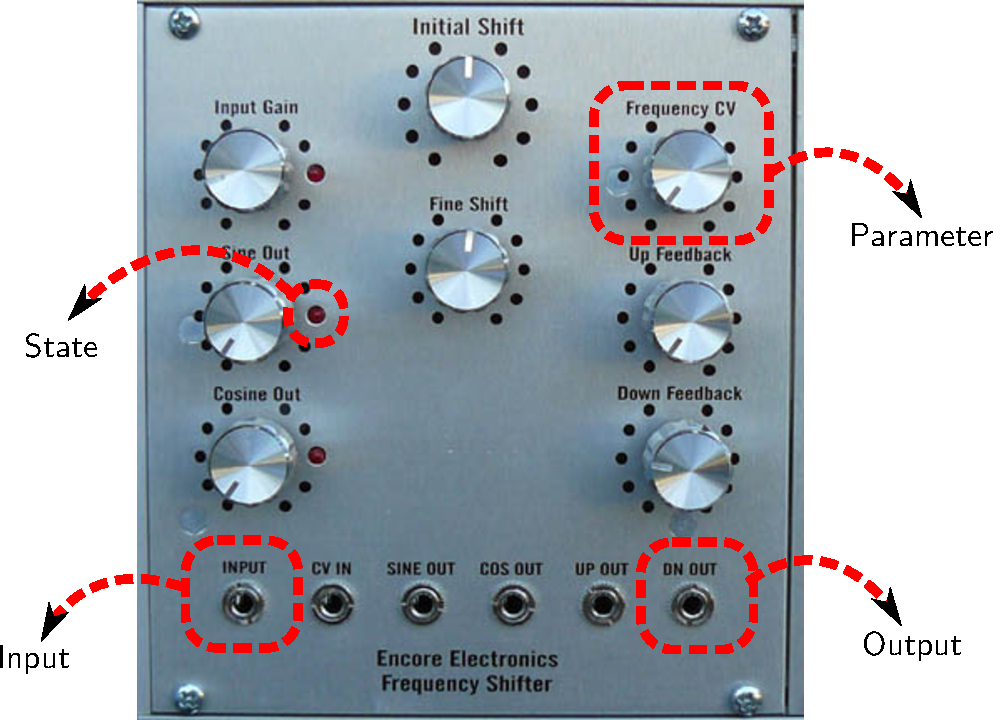
\includegraphics[width=.9\textwidth]{pic/hwmod.pdf}
  \caption{Components of a synthesis module illustrated in a standard
    \emph{frequency shifter}.}
  \label{fig:hwmod}
\end{figure}

A collection of modules and the connections among them is called a
\emph{patch}\index{patch}. In a hardware modular synthesiser, these
are assembled in special racks that have slots satisfying some
standard to place the modules in them --- for example, the module in
the figure fits in \emph{eurorack} slots. In many software synths, and
specifically in the one we are developing, patches can be arranged
hierarchically. We can visualise this as if we could put a whole rack
into a black box with holes to expose certain controls and ports to
the outside, and then place this box in a larger rack. This is very
useful in a software synthesiser; for example, one could build a
complex patch out of low-level processing primitives and expose a
simplified interface. Some software, like Reaktor, call these patches
\emph{instruments}\index{instrument}. This arrangement can then be
stored into a file for later use. On the Internet it is easy to find
many collections of these ready-to-use patches, and there are even
commercial packages developed by professional sound designers.

The \emph{conceptual class diagram} in figure \ref{fig:graphconcept}
summarises all this. Note that this is a conceptual class diagram, not
a design one, so there is not a direct match to the
classes in the actual code, not even terminologically.

\begin{figure}[h]
  \centering
  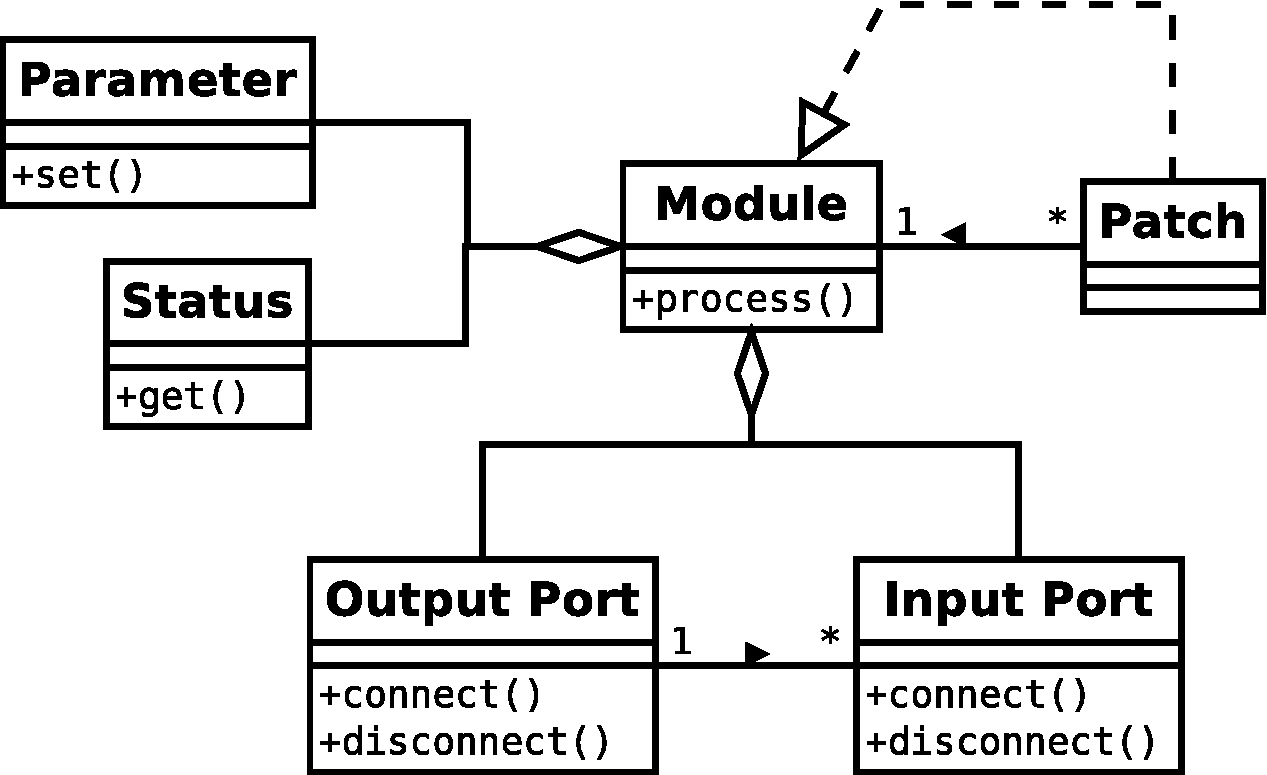
\includegraphics[width=.8\textwidth]{pic/graph-concept.pdf}
  \caption{Conceptual class diagram of the modular synthesis main
    entities.}
  \label{fig:graphconcept}
\end{figure}

\subsection{Software real time synthesis concerns}
\label{sec:rtsynth}

Our system generates the audio in real-time\index{real-time} sending
it directly to an output device --- a sound-card. Even more, it is
specially targeted at live performances, so every operation should be
designed such that it does not disrupt the audio generation process
and generates no kind of noise. For example, in some software modular
synths changing a connection among ports triggers a recomputation of
the dependencies among modules to generate a compiled form of the
patch for easier execution. But that often that takes long enough to
produce a small buffer underrun\index{underrun} --- i.e. an audible
click --- as it might involve doing non-linear computations or locking
certain mutexes to synchronise the state with the user
thread. Actually, the port reconnection issue requires special care,
as we will discuss in section \ref{sec:modports}. Because of
\emph{dynamic-patching}\index{dynamic-patching}, we should expect the
topology of the synthesis graph to change a lot during a live
performance.

To better understand this problem we should study how audio is
usually processed in real-time, thus feeding us with proper
terminology and knowledge to later tackle the issue. While this might
seem like a design issue to some, this is such a universal structure
that it shall be consider a fixed constraint to be analysed than a
design decision itself.

Ideally, we would produce each sample one at a time and send it to the
output device.  Traversing all the synthesis system for every frame
involves many function calls, some of them even require dynamic
dispatch in an extensible system like ours, leading to a too low
performance to deliver the samples on time --- in a consumer quality
system, we would need to produce 44000 samples per second! For this
reason, audio is processed blocks of \emph{block size} samples in
tight loops. This \emph{block size}\index{block size} might match the
device's buffer size\index{buffer size} or it might be
smaller. 

Parameter and status values are updated only in between blocks. Hence,
we should try to keep the block size as low as possible to avoid
noticeable latency, and most professional audio software allow
changing this parameter to fit the machine's processing power. A
sensible block size is 64 samples, like Pure Data's default. Using the
terminology in \cite{boulanger10audio}, we can distinguish between
\emph{audio rate}\index{audio rate} --- i.e. the frame rate as
described in the previous chapter --- and \emph{control
  rate}\index{control rate}, which is the sampling frequency of
control signals --- i.e. the signals that produce only one sample per
processing block:
\begin{equation}
  control\_rate = \frac{audio\_rate}{block\_size}  
\end{equation}

Note that control signals are not restricted to what we labelled as
\emph{controls} in the previous sections. In fact, through a
\emph{port} signals may flow at audio rate if their signal type is
that of an audio buffer that holds a block of samples, or at control
rate if their signal type is that of a single sample, like a
\type{float} or \type{double}.

Interleaving the sound generation within the user-interface loop is
not plausible; thus the audio processing lives in its own thread/s. In
fact, as we saw in the last chapter, some audio output interfaces like
Jackd control the audio thread themselves invoking the processing
function through a callback. Our own device API wrapper that was
developed in the previous chapter promotes this kind of asynchronous
output and simulates it whenever the output system only provides a
blocking I/O interface. The inverse of the control rate, that we may
call the \emph{control period}, provides a very explicit deadline for
the block processing function. Missing the deadline might not kill
people, but it would produce an unpleasant clicking noise and thus we
have to do as much as possible to meet the deadline\footnote{In fact,
  in the middle of a live performance with a $10^5$ watts sound
  system, consequences can be more severe as it may seem superficially
  ...}. Hence, our system can be categorised as \emph{soft real-time}
\cite{tanenbaum07mos}. This implies that, apart from trying to get
real-time priority in the audio thread, we have to take special care
when developing the program, and this will deeply influence the
design:

\begin{enumerate}

\item Avoid system calls in the audio thread. System calls produce a
  context switch and it can take quite long until the audio thread is
  preempted back; at least too much to meet the deadline. This is
  specially true for I/O system calls. In the previous chapter we
  already provided some devices to avoid this problem, like the
  caching file readers.\index{system call}

\item Avoid contending for a \emph{mutex}\index{mutex} or some other
  kind of lock with the user thread. Without special support from the
  operating system --- like priority inheriting mutexes --- this can
  lead to priority inversion \cite{kim03basic}. Even in the later
  case, the context switch produced by the contention gives good
  chances to miss the deadline until the audio thread is
  preempted. The overhead of locking a mutex when there is no
  contention is negligible in most operating systems, and it
  definitely is in Linux which uses \emph{futexes} (Fast User-space
  Mutex) to implement them \cite{franke02futex}, so using a
  \emph{try-lock} operation is usually acceptable. The rule of thumb
  is to never wait on a mutex in the audio thread, and use lock-free
  data structures \cite{valois96lockfree} or do conditional locking
  instead.\index{priority inversion}\index{lock-free algorithm}

\item Because the deadline depends directly on the block size $n$,
  algorithms running in the audio thread\index{audio thread} should be
  in $O(n)$. A special consequence of this restriction is that
  allocating memory in the heap\index{heap allocation}, at least with
  the default allocator --- i.e. using \type{new} --- is
  forbidden. This is so because memory allocation algorithms are not
  proportional to the size of the requested block, but instead depend
  on non-deterministic properties --- like the pattern of memory usage
  --- and use complex search algorithms to find a fitting block of
  spare memory. This restriction implies that manipulating STL
  containers is forbidden too. For some special kinds of objects, like
  same-sized objects, a custom memory allocator can do the job
  \cite{alexandrescu01modern}. Sometimes, an intrusive data structure,
  like \emph{Boost.Intrusive} STL counterparts
  \footnote{\url{http://www.boost.org/doc/libs/release/doc/html/intrusive.html}}
  are enough to avoid the allocations. In other situations, we can
  release the job of allocating memory to the user thread, use custom
  data structures or any other ad-hoc solution.
\end{enumerate}

\subsection{Anticipating future needs}

For the sake of proper workload balancing, several features that
deeply affect the structure of this layer are delayed for later
development iterations. However, to prevent rewriting the code at
those stages, we should anticipate what characteristics are
required from the basic constructs in order to later extend the system
with such features.

\subsubsection{Polyphony}

\index{polyphony}Polyphonic audio allows building chords and enrich
the whole harmonic depth of the music
\cite{johnson02measured}. Polyphony is produced when several notes are
played at the same time; for example, by pressing simultaneously
several keys of a keyboard. Actually, polyphony is also present
without simultaneously pressing several keys, as instruments usually
have a significant \emph{decay time}\index{decay time} --- i.e. the
time between the key release and the sound fully fades out ---
blending the sounds of successive key strokes.

Because in a modular synthesiser a generator is producing a single
tone at a time, it is not trivial to implement polyphony. In practise,
several copies of the processing graph are to be maintained, each one
is called a \emph{voice}\index{voice (polyphony)}. When a new note is
to be played, the system has to allocate a voice for it and trigger
the processing; when the key is released and the note fully faded out,
the voice is released. Voice allocation is in many ways similar to
other allocation mechanisms, like page allocation in an operating
system, and different stragies have been proposed: \emph{round-robin},
\emph{last-in-first-out}, \emph{priority based algorithms}, etc. The
number of of voices is called the \emph{level of polyphony}, which is
usually user-controllable but fixed during a performance parameter of
the system. Modern computers allow levels of polyphony
high enough (from 16 to 128) such that the sophistication of the
allocation mechanism is not too relevant for the overall qualitative
experience of the sound produced by the synthesiser. Also, in a
modular software synthesis engine, a whole network needn't be
polyphonic. For example, some dynamic range compression or reverb
filters are usually applied to the final mixed sound of all voices,
yielding not only better performance but also a richer sound.

It is not worth to concentrate on the actual management of the
different voices and the triggering mechanisms until sequencing and or
MIDI support is developed in later stages. However, there are some
questions that we do have to address now:
\begin{itemize}
\item We have to split the responsibilities of the different classes
properly predicting which classes will need to be extended, preferably
via inheritance, to provide the polyphony support.

\item We have to define, at least partially, an interface that
  polyphony enabled DSP nodes will have to implement.
\end{itemize}

\subsubsection{Plug-in system}

At a later stage, we plan to implement a plug-in\index{plug-in} system
as defined by requirements \ref{req:iter3-begin} to
\ref{req:iter3-end}. These plug-ins shall be in several formats, like
LV2\index{LV2 (plug-in)}, LADSPA\index{LADSPA (plug-in)}, or our own
defined interface. We should take this into account in several ways:
\begin{enumerate}
\item For consistency, the interface for implementing modules that we
  will define in this chapter shall be the same that our own plug-ins
  will implement later. The only significant difference should be the
  linking method of the code and the registration mechanism.

\item Even for statically linked DSP modules, bject construction
  should be done in an indirect way, via object
  \emph{factories}\index{factory (design pattern)}
  \cite{gamma95design}. Thanks to this, the system can later be
  transparently extended by modifying the factory manager to delegate
  the construction of specially-identified objects --- objects
  identified by a resource URI \cite{mealling02rfc3305} --- to a
  plug-in loader.

\item Parameters, states, inputs and outputs of an object should be
  accessed via dynamic means of introspection. In practise, they
  should be identified by strings ands modules should provide some way
  of iterating through them. Ideally, there should be some hooks to
  provide some meta-data that can be useful for an automatic user
  interface builder; for example, a parameter's range, whether it is
  naturally linear or logarithmic, etc.
\end{enumerate}

\section{Design}

\subsection{Overview}

Figure \ref{fig:graphoverview} shows an overview of most important
classes in this layer from the musical point of view. Most of the code
implementing these classes lives in the \type{psynth::graph}
namespace, named after the fact that this layer implements the notion
of sound processing described as a graph of interconnected processing
modules. The \type{node} class is the base class of all kinds of
vertexes in this graph. Therefore, \emph{node}\index{node} is a
synonym for what we called \emph{module}\index{module} or \emph{DSP
  node}\index{DSP node} in the analysis section; i.e. it is the basic
unit that processes some input signals producing new output values. In
the rest of this chapter, unless otherwise stated in its close
context, we will use the term node with this meaning.\footnote{Indeed,
  we prefer this term as the name \emph{module} has a different
  specific meaning in the code, similar to that of \emph{translation
    unit}.}

\begin{figure}[h]
  \centering
  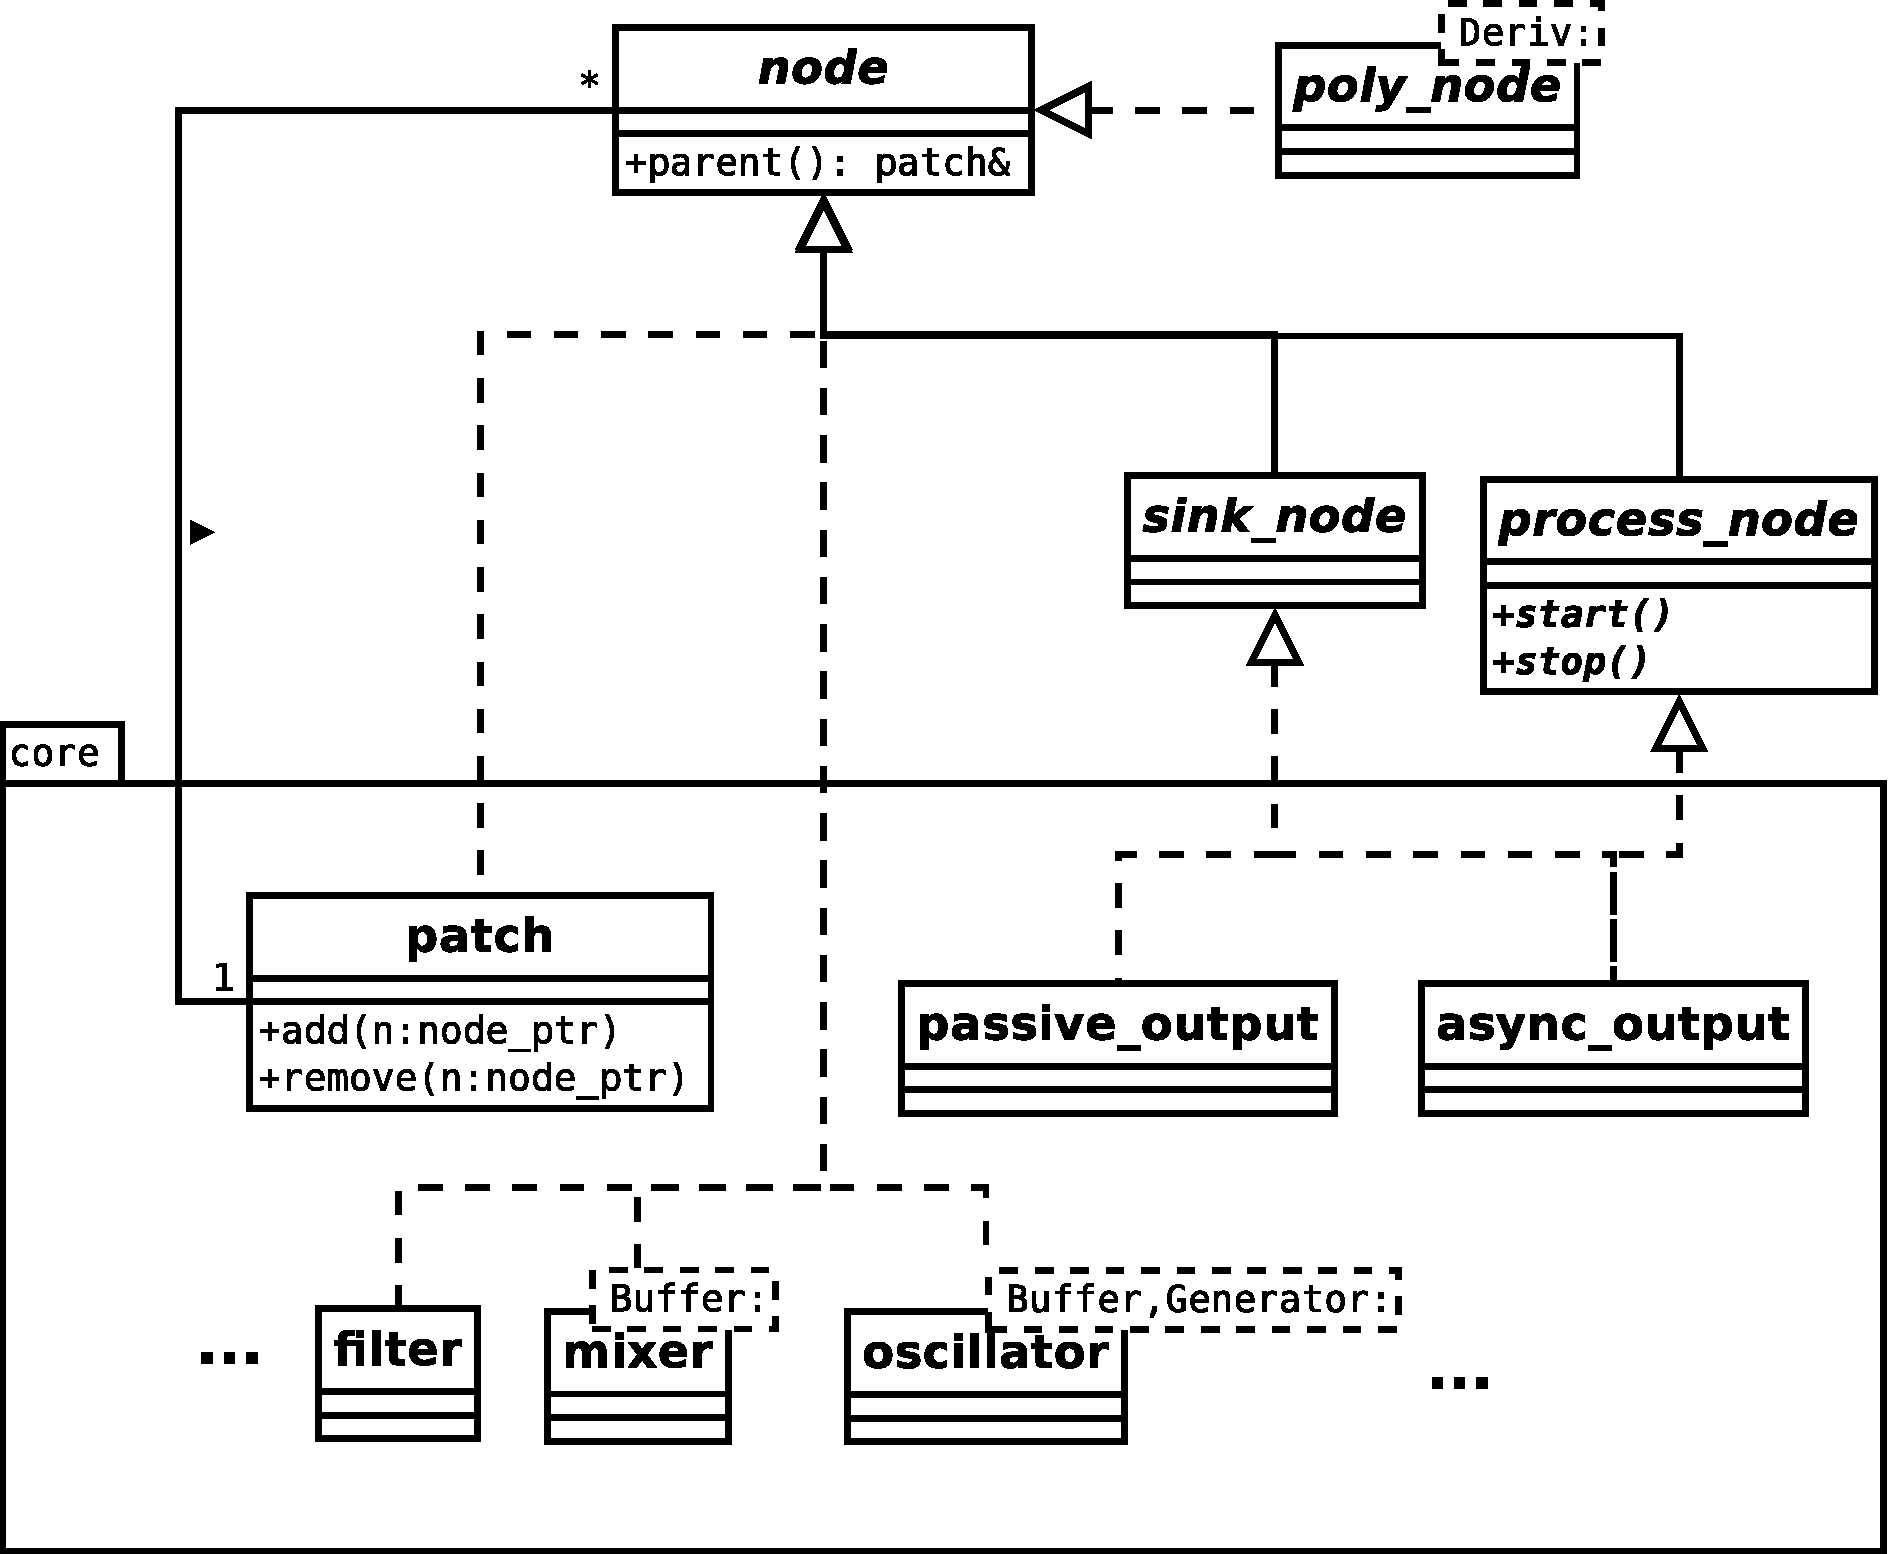
\includegraphics[width=\textwidth]{pic/graph-node.pdf}
  \caption{Overview of the graph layer}
  \label{fig:graphoverview}
\end{figure}

The \type{psynth::graph::core} namespace contains the \emph{concrete}
nodes that are implemented in our library. All these shall be
registered in the object factory that we will describe in section
\ref{sec:graphfactory} and most of the code should not instantiate
these modules directly. This introduces the notion of \emph{core
  node}\index{core node}, i.e. a node that is built-in --- statically
linked --- inside the library, thus it is not a plug-in. Other sorts
of abstract nodes that are there only to offer certain basic
functionality should live directly in the \type{psynth::graph}
namespace, and they are considered basic infrastructure and may be
useful in the implementation of plug-ins.

We will explain other parts of this diagram later. What should be
clear now is the relationship between a \type{node} and a
\type{patch}. This is an instance of the \emph{composite} design
pattern \cite{gamma95design, vlissides98pattern}. A \emph{patch} is a
collection of nodes but it is a node by itself, building tree-like
structures that most of the time have non-patch nodes as leafs, and a
patch on its root. To ease memory management, \type{node\_ptr} is an
alias for \type{std::shared\_ptr<node>}\footnote{This is a recurring
  pattern, also explained in the ``Programmer guide''.}. A node keeps a
weak reference to its parent easing traversal and some special
operations, accessible via the \type{parent ()} method.

We will next explain the execution model of the synthesis network
defined by these classes, but first, lets make a parenthesis to
explain a novel data-structure that is deep in its core.

\subsection{Heterogeneous deques --- bridging polymorphism and
  real-time processing}

As we explained in the analysis section, avoiding heap allocation is
crucial in real-time processes\index{real-time}. Proper runtime
polymorphism\index{polymorphism!dynamic} is said to require heap
allocation\index{heap allocation} because the code paths in charge of
managing the lifetime of some object do not know its full type ---
specially the actual object size --- and thus the object can not be
allocated in the stack. While true in general, we can constrain the
problem in several ways to obtain $O (1)$ allocations if the
programming language provides enough low level constructs to implement
these solutions.

A possible solution is to override the operator \type{new} for certain
types to provide constant-time allocation. Alexandrescu provides a
clever way of doing this \cite{alexandrescu01modern}. This,
however, have several problems:

\begin{enumerate}
\item \emph{Concurrency}. We have, in general, several threads
  creating objects of these kinds. Alexandrescu solves the problem by
  using mutexes. This is forbidden in our real-time thread; which is
  just what we are trying to avoid. Maybe a lock-free data-structure
  could be used to allocate this memory, solving the issue, but we do
  not any that would fit this purpose.

\item \emph{Explicitness}. We would like to easily know what
  operations are safe to be performed in the real-time thread. Any
  programmer should get worried when she reads something like this in a
  real-time code path:
  \begin{lstlisting}
    some_type* x = new some_concrete_type (...)
  \end{lstlisting}
  To regain confidence about the correctness
  of that code, she should go and read the implementation of
  \type{some\_\-concrete\_\-type} and discover that it has an
  overloaded operator \type{new}.
\end{enumerate}

Another plausible solution is to constrain the set of types acceptable
in some variable. By doing so we are, in fact, changing the open world
assumption of universal polymorphism\index{polymorphism!universal} by
the closed-world assumption of ad-hoc polymorphism. Thanks to this
constrain, we can, via template metaprogramming or the new C++11
\texttt{constexpr} facility, compute at compile time the maximum
storage needed to hold values of any of those types and allocate it in
the stack; then construct the objects in this space with
\emph{placement new}. This is actually how \index{variant}
\emph{Boost.Variant}\footnote{\url{www.boost.org/doc/html/variant.html}}
is implemented \cite{alexandrescu01unions}, and as we are depending on
Boost already, using it is quite safe in real-time code and can be a
solution when ad-hoc polymorphism is enough.\index{polymorphism!ad-hoc}

In some other cases ad-hoc polymorphism is not enough, but the pattern
of object construction and destruction can be constrained instead. We
can think of \emph{the heap} as a global data-structure --- a
data-structure that is so useful that its insertion and deletion
operations are keywords of the language itself --- i.e. the global
operators \type{new} and \type{delete}. In fact, its interface is very
similar to that of a multi-set, but without iteration and with the
ability to hold elements of varying size. If we restrict its interface
such that elements can only be allocated and released in FIFO or LIFO
order, we get a \emph{deque}.

\begin{lstlisting}[float=h!,caption=Example of usage of heterogeneous deques,label=lst:heteroexample]
  struct base {
      virtual void method () { std::cout << "b"; };
  };
  struct deriv : base { 
      deriv (int x = 0)      {} 
      virtual void method () { std::cout << "d"; };
  };

  hetero_deque<base> q;
  base b;
  deriv d;

  // 1. Copying
  q.push_back (b); q.push_front (d);

  // 2. Moving
  q.push_back (deriv ()); q.push_front (std::move (b))

  // 3. Constructing, even with params!
  q.push_back<base> (); q.push_front<deriv> (1);

  // Error checking
  // static_assert error: 'int' is not a subtype of 'base'
  q.push_back (1); 

  // Access is polymorphic!
  // Output: bddbbd
  for (Base& x : q)
    q.method ();
\end{lstlisting}

\index{heterogeneous deque}The class
\type{psynth::\-ba\-se::\-he\-te\-ro\_de\-que<Base>} is a
cons\-tant-size deque that can hold elements of any subclass of its
type parameter \type{Base}. The concrete type of the object must be
known at insertion time for the deque to be able to allocate space for
it in its internal buffer. Actually, the data structure API offers
three ways of inserting a concrete derivative of \type{Base} into it:
(1) copying it, (2) moving it using R-value references or (3) directly
constructing it into the data-structure, using perfect forwarding to
pass the parameters. The inserted element must be a subtype of
\type{Base} and this is statically checked rising a
\type{static\_assert} error otherwise. All this is illustrated by the
example in listing \ref{lst:heteroexample}.

The data-structure interface is similar to that of an STL deque, with
some differences. Because access is done polymorphically via a
reference of type \type{Base\&}, \type{value\_type} semantics, which
maps to \type{Base}, are slightly different than in most containers
because the actual elements are of different heterogeneous concrete
types. Also, because objects can be directly constructed inside the
data structure with arbitrary parameters, they needn't be regular in
any sense, this is, they don't have to be copy-constructible,
move-constructible, default-constructible, copyable or moveable. This
is quite convenient because classes that are designed to be used
polymorphically, more often than not, they do not satisfy many of these
properties. The only restriction is that \type{Base} should have a
virtual destructor if any of its derivates has a non-trivial
destructor.

Note that the data structure itself is not copyable, nor moveable, nor
resizeable. While it would be feasible to implement it otherwise, it
has a slight memory overhead. As our current use-cases do not need it,
we decided to stick to the current simpler implementation. This is so
because to be standard compliant, an object identity --- i.e. the
memory address where it lives --- must remain constant during its
livetime; in order to copy or move it, we need to call the proper copy
or move constructor, and in the later case call the destructor of the
moved object if it is to be released \cite{cppstd}. Calling the proper
copy or move operation requires, at least, one function pointer --- or
a \emph{vtable} pointer for a box type. We already have a plan to
implement this feature using \index{policy-based design}policy-based
design \cite{alexandrescu01modern} so it would not cause an overhead
to those who do not need it.

\begin{lstlisting}[float=h!,caption=Header of heterogeneous deque elements,label=lst:heteroheader]
  template <class Base>
  struct header {
      header* prev;
      header* next;
      Base* access;
  };
\end{lstlisting}

The data structure is implemented by storing the objects in a constant
sized memory block organised in a circular buffer fashion.  We append
a header like the one in listing \ref{lst:heteroheader} at the
beginning of each a object. An empty header at the end of the list
allows to keep track of the beginning of the free space. The
\type{prev} and \type{next} pointers organise the data in the deque in
a doubly-linked list fashion. Even though the storage is continuous,
this is needed because the size of the objects is variable and only
known at object insertion time. The \type{access} pointer keeps a
reference to the object itself casted to \type{Base*}. This is
required because, in the presence of multiple-inheritance, the
\type{Base} part of the object might not be aligned at the beginning
of the object's layout. If we think about it, the \type{next} and
\emph{access} pointers are just a way of keeping track of the
static information that is lost in the \emph{type erasure}
that happens when adding a new element to the data structure: its
\emph{size} and the \emph{offset} to its still known attributes and
\emph{vtable}; the \type{prev} pointer just aids reverse traversal and
addition at the front.

Figure \ref{fig:heterostructure} represents an instance of the data
structure containing two objects. The \type{front} and \type{back}
pointers keep track of the first and last valid element in the
container. We can see how adding a new element that does not fit at
the end of the memory space, causes that space to be wasted --- marked
as \emph{offset} in the figure --- and the object is instead added at
the beginning of the memory block, where there is enough free space
available in this case, in a circular buffer fashion.

\begin{figure}[h!]
  \centering
  \subfloat[]{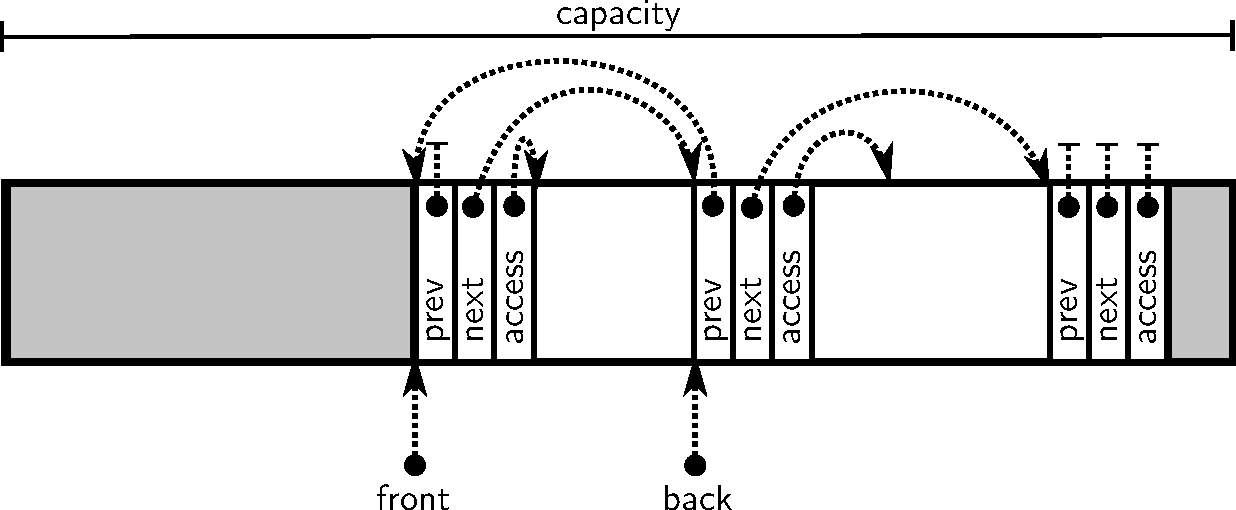
\includegraphics[width=.95\textwidth]{pic/hetero1.pdf}}

  \subfloat[]{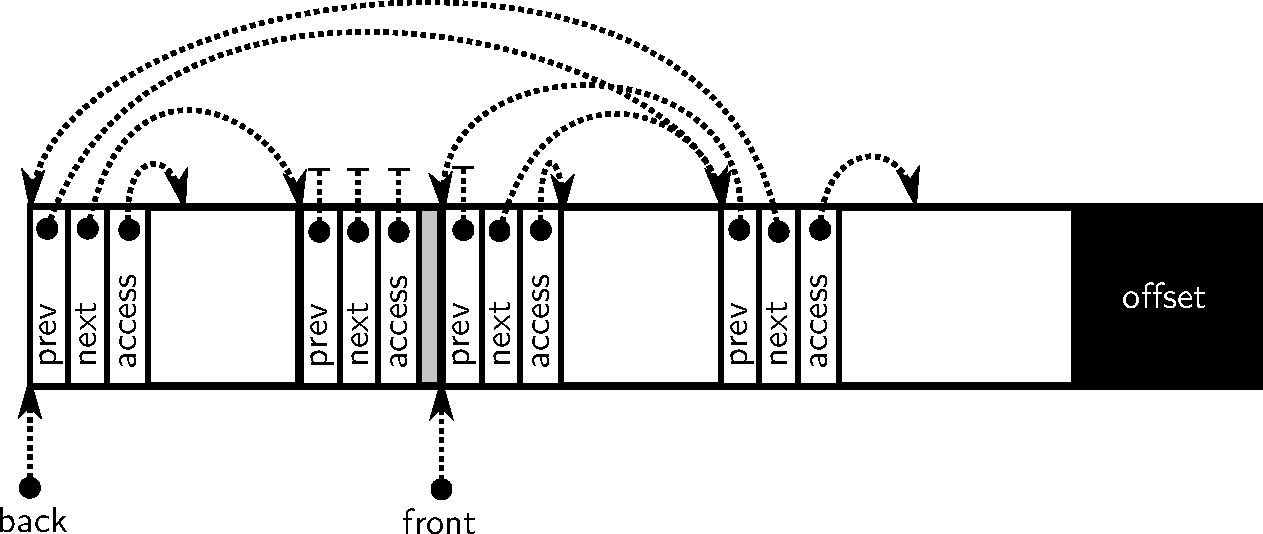
\includegraphics[width=\textwidth]{pic/hetero2.pdf}}

  \caption{An heterogeneous deque with two elements (a), and after
    adding a third element (b).}
  \label{fig:heterostructure}
\end{figure}

So, thanks to low level facilities provide by C++, we are able to use
different techniques to get the benefit in expressiveness and
maintainability of polymorphism in a real-time constrained
environment. Our most prominent use-case, passing active events among
different threads, gets very benefited from our last approach, as we
shall see in the rest of this section. In other parts of the system,
\index{disjoint union}disjoint unions as implemented by
\emph{Boost.Variant} are enough, and we actually do use them, for
example, to treat a closed family of oscillator objects
polymorphically in our oscillator node implementation. A custom object
allocator is a valid solution in some other situations, but as we have
already analysed, it is mostly unsuitable for our quite specific
needs.

\subsection{Execution model}

\begin{figure}[h]
  \centering
  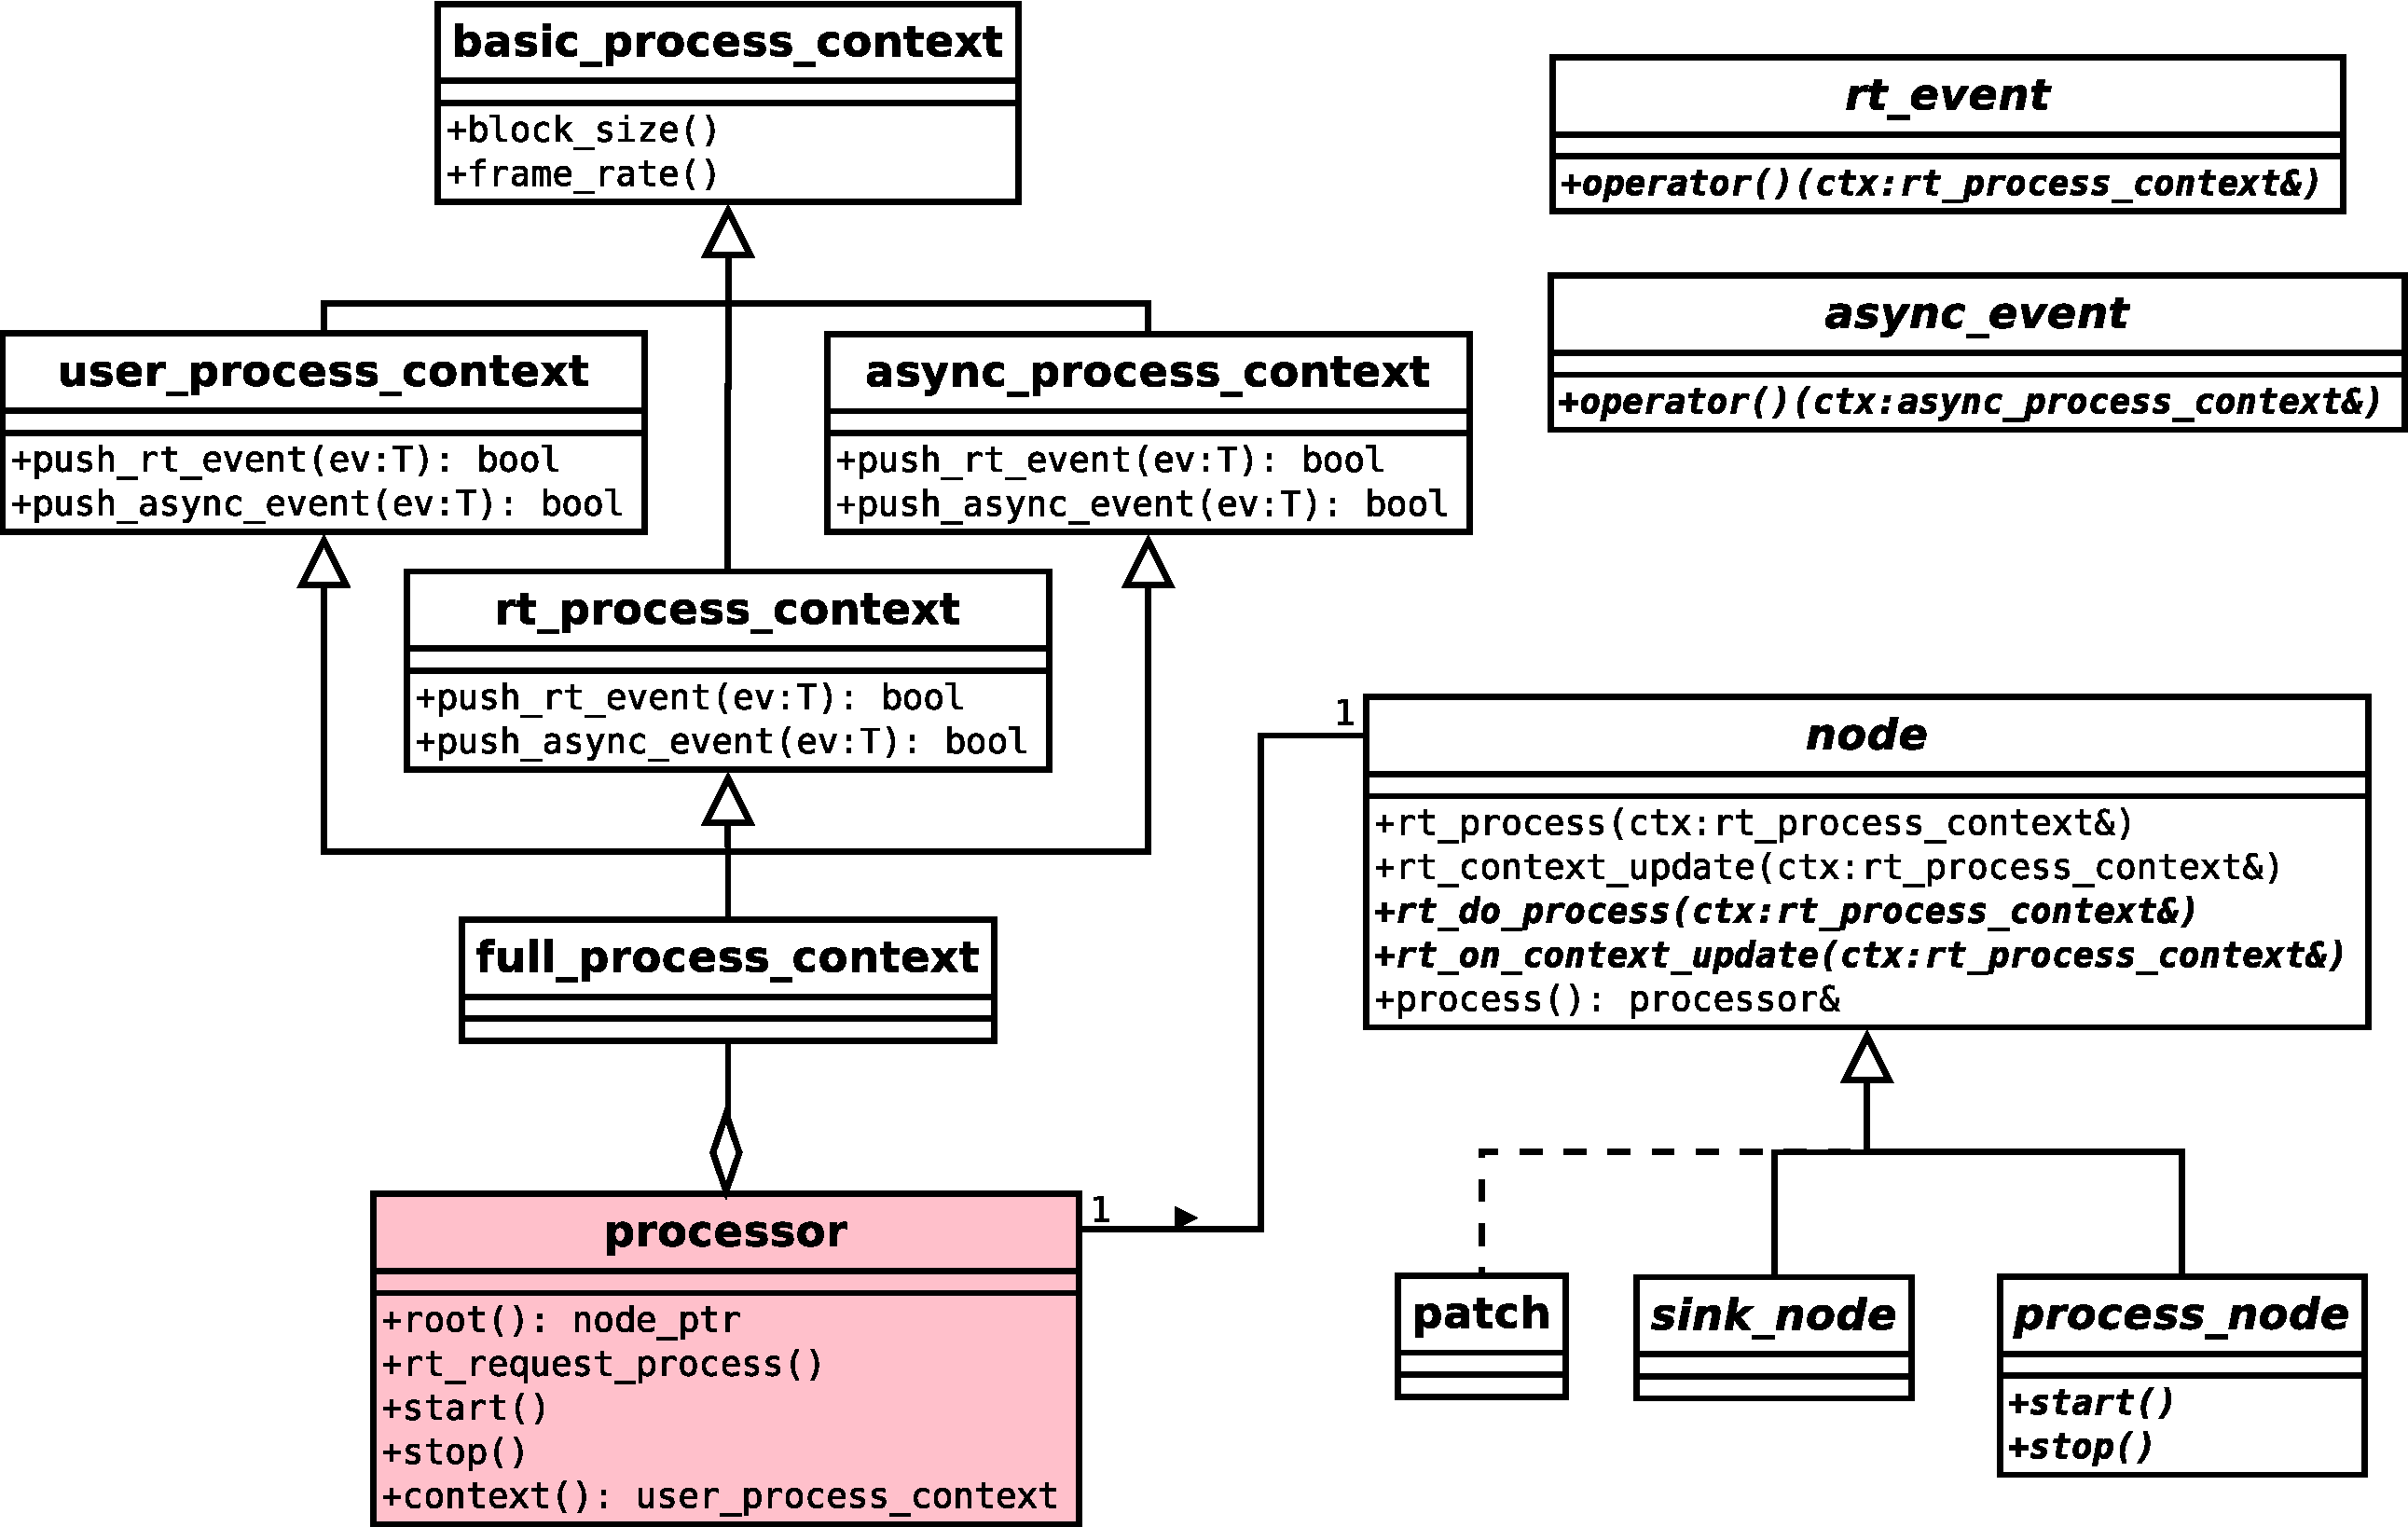
\includegraphics[width=\textwidth]{pic/graph-processor.pdf}
  \caption{The graph processor, its context and the processing methods
    of nodes. }
  \label{fig:graphprocess}
\end{figure}

Figure \ref{fig:graphprocess} introduces some new classes that are the
coordinate the execution of the synthesis graph. Because there are
several concurrent --- and potentially parallel --- threads of
execution, writing code without race conditions and other
synchronisation problems can get quite hard if we do not establish
some conventions. Unless otherwise specified in its documentation, a
method is expected to be executed in only one \emph{kind} of thread,
sometimes even in just only one specific thread. There are three kinds
of threads and some naming conventions allow us to determine in which
thread some method is expected to be used:

\begin{description}
\item[User thread]\index{user thread} The user thread is the one where
  most objects are created and where, usually, the user interface
  lives. In some way, this can be considered the \emph{normal thread},
  and it is the root of the thread tree --- i.e. the one that creates
  the other threads.

  If a method does not have any special prefix nor belongs to a class
  named with a special prefix, we shall assume, unless otherwise
  specified in its documentation, that it is safe to execute it only
  in the user thread. In the current implementation, these methods,
  while reentrant, they are not fully thread-safe. This means that
  most non-const methods of an object and related objects
  --- i.e. objects that keep references among themselves --- shall be
  executed in the same thread, but it is safe to operate with
  unrelated objects in different user threads.

\item[Real-Time (RT) threads]\index{RT thread}\index{audio thread}
  These are the threads where the actual work of processing the
  synthesis graph is done. We sometimes call these just the
  \emph{audio thread}. As we shall see later, these threads are
  controlled by the \type{process\_node} derivates, but that is not
  relevant now. Methods beginning by the \type{rt\_} prefix, and all
  methods of classes named with that prefix, are expected to be
  executed in this thread. While it can be normal for several RT
  threads to coexist, implementers of RT-methods and objects should
  not worry about this, because, unless they are actually implementing
  a \type{process\_node}, the system itself serialises calls to
  dependent methods --- in the current implementation, it just
  serialises calls to \type{rt\_request\_process}, we will discuss
  this further soon.

\item[Asynchronous operation threads] \index{async thread}These
  threads, that we may call just \emph{async threads}, ease the
  execution of operations that are forbidden in the RT thread. The
  \type{processor} controls the execution of these threads. Methods
  and classes prefixed with \type{async\_} are expected to be executed
  in these thread.
\end{description}

\subsubsection{Processing the graph}

The \type{processor} class is a \emph{facade}\index{facade (design
  pattern)} that manages the execution of the synthesis graph
described by a given root node. Of course, a whole graph can be
attached to one and only processor and an exception would be thrown if
we try to attach it to several.

\begin{algorithm}
  \caption{Process a control iteration of the graph, $rt\_process (n,
    ctx)$}
\label{alg:processgraph}
\begin{algorithmic}
  \REQUIRE $\;$\\
  $n \in \mbox{\type{node}}$ \\
  $ctx \in \mbox{\type{rt\_process\_context}}$
  \ENSURE $\;$\\Every node in the graph is processed and its results ready in their
  outputs, if any, in the right order.
  \medskip
  \IF{$\lnot visited (n)$}
  \FORALL{$i \in inputs (n)$}
  \IF{$connected (i)$}
  \STATE $n_i \gets source (i)$
  \STATE $rt\_process (n_i, ctx)$
  \ENDIF
  \ENDFOR
  \STATE $rt\_do\_process (n, ctx)$
  \STATE $visited (n) \gets \top$
  \ENDIF
\end{algorithmic}
\end{algorithm}

The \type{rt\_request\_process} method triggers the execution of one
iteration of the graph processing, this is, it processes one block of
audio rate samples or one control sample. The processing algorithm is
as follows. The processor keeps a list the nodes that have
side-effects outside the graph itself, for example, a node for
outputting to a device. These are the nodes that inherit from
\type{sink\_node}, and we can refer to them as just \index{sink node}
\emph{sinks}. For every sink, the processor invokes the recursive
algorithm \ref{alg:processgraph} implemented by \type{rt\_process} in
the \type{node} class. This recursively calls the process method of
the nodes connected to one's input. Because the synthesis graph may
have loops and input ports may be connected to several outputs, it
marks every node it visits. In this way, every node is processed only
once and nodes that may have no side effects are discarded --- because
they do not interact wit the ``real world'' nor any node that does
depends on it. When a node is being visited, the pure virtual
\type{rt\_do\_process} methods is invoked. That is the most important
method that implementers of their DSP modules have to take care of; in
it they should fetch the input data, if any, process it, and write
some output, if any. We often just call this the \emph{worker method}
of a node.

\subsubsection{Proactive nodes}

\type{rt\_do\_process} is usually executed by implicitly triggered by
\emph{process\_nodes}.\index{proactive node} These nodes represent
devices that may require processing from the graph, and they have and
extra \type{start ()} and \type{stop ()} methods. They are in charge of
managing their own thread where they request processing whenever they
need frames. The start and stop methods manage the status of this thread.

A canonical concrete \emph{process\_node} is
\emph{core::async\_output}, which, when associated to an asynchronous
output device (see section \ref{sec:asyncio}), requests processing in
the output callback and passes what it gets from its single input port
to the device. In order to allow several asynchronous output devices,
calls to \type{rt\_request\_process} are serialised. Then, in their
worker method they just accumulate their input in an internal ring
buffer, but they do not directly output to the device, because that
operation may block and delay other devices that are waiting on this
request. In their own device callback, when there is enough
information in their internal ring buffer, this is sent to the device.

Calls to \type{rt\_request\_process} are serialised using a mutex in a
special way. When we try to get the lock and it is owned already, we
do wait for the ongoing request to finish but we do not perform a new
request, because the one that was already on the way might have been
enough for the device to get sufficient information. This use of locks
does not violate the RT rules, because all threads that are expected
to contend for it are real-time so no priority inversion can occur. It
may introduce some context switches, but that is unavoidable, and in
practise they do not add much overhead, and in modern processor the
gained parallelism compensates. While we are doing the output
operation on the device, another process node might have triggered
another request, preparing our next bunch of frames already. When we
are locked on the mutex, another RT thread is already doing what we
wanted to do, and if the OS scheduler is not dumb, it should preempt
our RT thread soon at it will happily find that its request have been
processed already. Thanks to this mechanism we can output to several
devices at the same time, even if they are in different sound
cards. What information is set to each one depends on how the graph is
interconnected, and it might even be different, of course. This is a
common usecase, for example, DJ's peek at how the next track mixes
in while they adjust its tempo on their headphones without altering
what is still being played on the loudspeakers. Figure
\ref{fig:djscheme} shows how a typical DJ setup could be built with
Pyschosynth's engine and illustrates the most important aspects of the
algorithm that we just described.

\begin{figure}[h!]
  \centering
  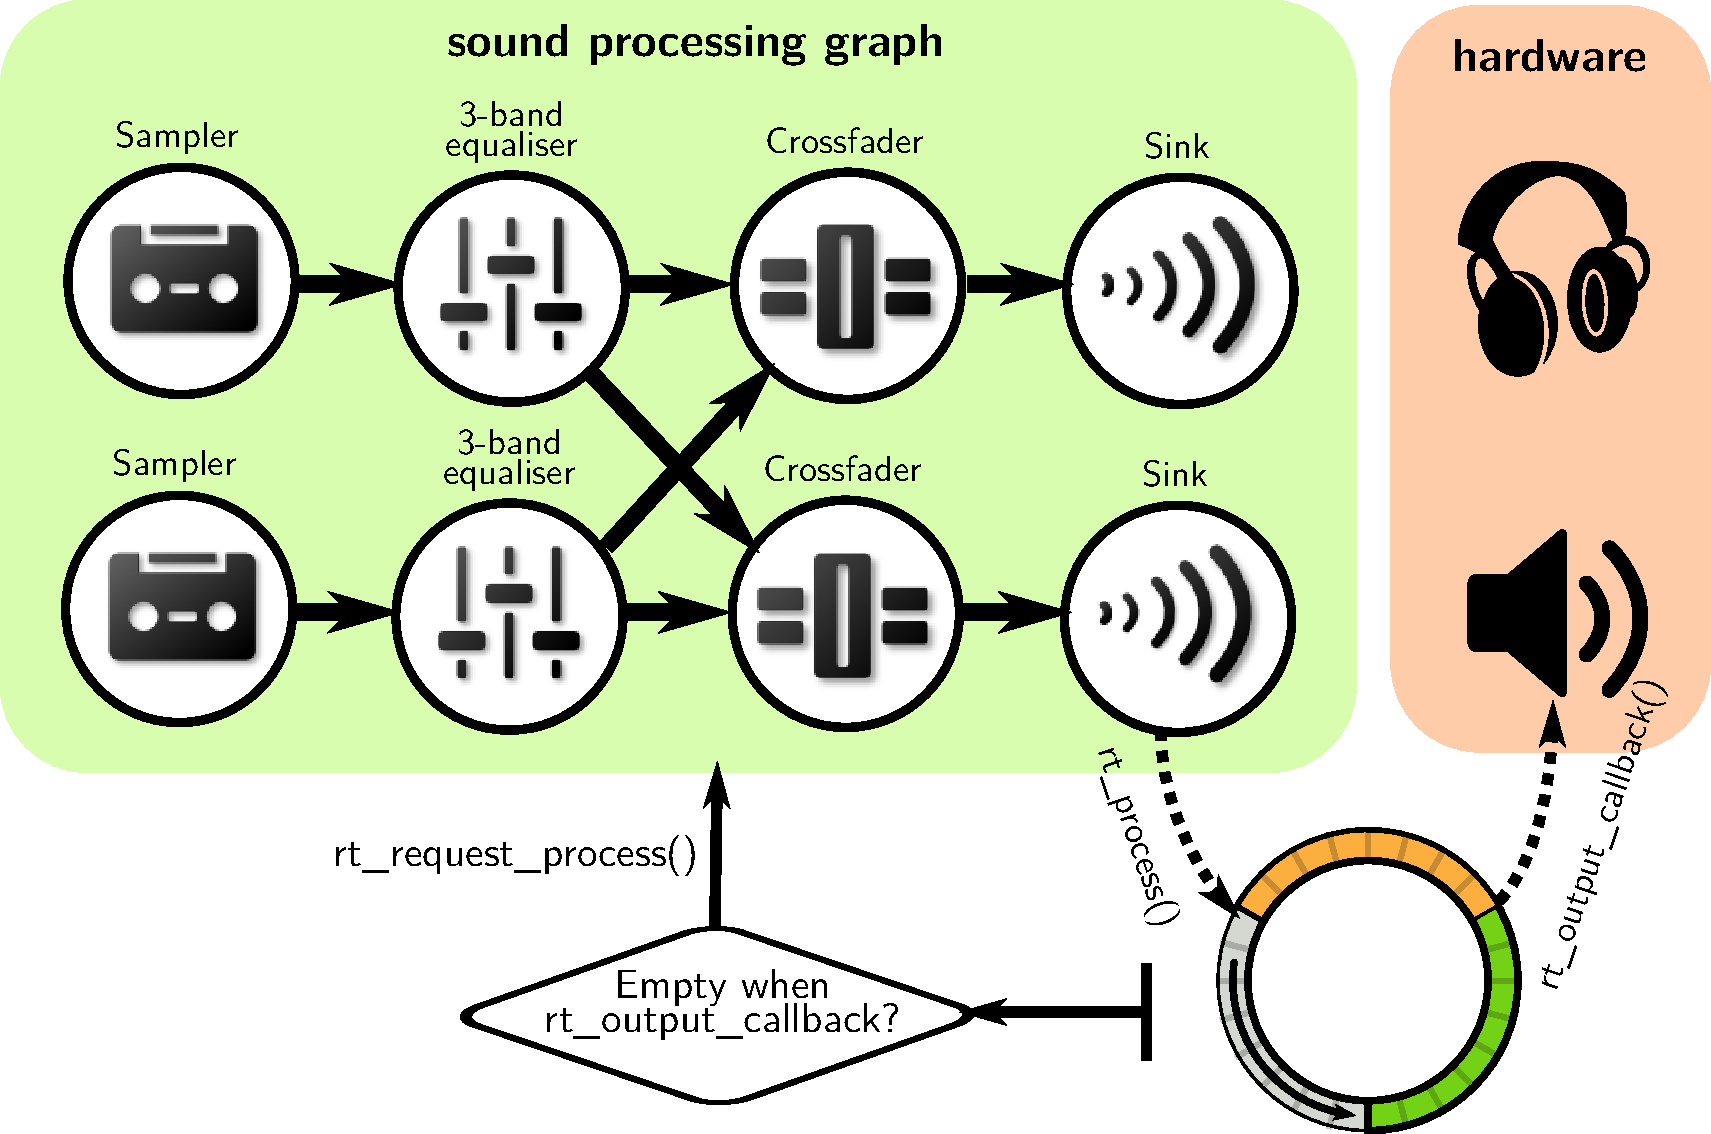
\includegraphics[width=\textwidth]{pic/djscheme.pdf}
  \caption{A DJ setup built with Psychosynht's engine to illustrate
    the multiple device output system.}
  \label{fig:djscheme}
\end{figure}

The \type{start ()} and \type{stop ()} methods in the \type{processor}
class are in charge of starting and stopping all the process nodes in
its associated graph. This class also starts nodes that are added
after the processor have already been started and stops them when
removed. Usually, we can just start the processor at the beginning of
our program and start manipulating its graph. These methods also
control the execution of the \emph{async thread}.

\index{passive node}For completeness, we shall mention that there are
passive output nodes that only write data in the event of an external
request for processing. We can use this, for example, to record a live
session driven by a second active device to a file. Also, if we only
want to generate the audio directly in the file without the presence
of any proactive sink, we may directly call
\type{rt\_process\_request} in the user thread as many times as
needed, taking into account that the duration of the file resulting
from calling it $i$ times is, in seconds:
\begin{equation}
  duration(i) = \frac{i \times block\_size}{frame\_rate}   
\end{equation}

\subsubsection{Communication between threads}

Creating proper abstractions for communicating among the different
threads is essential for the extensibility of the system. This is, in
fact, one of the main flaws of the former implementation of this
layer. The usage of ad-hoc mechanisms for every different feature made
the system harder to understand, leading to subtle race conditions,
the overuse of locks and unnecessary busy-wait checks in the RT
thread.

It should be almost clear already why we need our own thread
communication abstraction instead of just using some traditional
blocking mechanism --- message passing, monitors, etc. First, the RT
threads should not wait on non-RT threads like the user thread or the
async threads. Moreover, most of the processing in the RT thread
should be done in tight, simple, loops; even if the parameters coming
from other threads where implemented with atomic variables, this state
should not change during the execution of these loops. What we do
instead is to delegate the execution of actions with side-effects
visible by another thread to that thread itself. We call these actions
\emph{events}\index{event}, and they are an instance of the
\emph{command} design pattern \index{command (design pattern)}
\cite{gamma95design}. Going back to figure \ref{fig:graphprocess}, we
can distinguish two kinds of events, \type{rt\_event}, that are to be
executed by the RT thread, and \type{async\_event}, that are executed
in the asynchronous thread. Note that there is no notion of
\type{user\_event}, because that would add unnecessary complexity. If
the async thread wants to produce side-effects visible to the user,
they can just coordinate using locks, because they are not forbidden
in the async thread. If the RT thread wanted to do so, he can just
send an event to the asynchronous thread that does the synchronised
update in that unconstrained environment.

The events are just functors with its overloaded \type{operator()}
made virtual. The \emph{fn\_*\_event} family of concrete events just
wrap a non-polymorphic functor to match the corresponding
interface. This recurring pattern of embedding a object with a
non-polymorphic interface into an adaptor with the same interface
implemented with virtual methods is called \index{boxing}
\emph{boxing}. The \type{make\_*\_event} family of box factories use
template argument deduction to automatically box its parameter without
explicitly writing its type. This is extremely useful with the new
C++11 lambdas, because to have a compile-time determined
size\footnote{Something that gracefully allows us to use them even in
  our RT-thread as long as we do not erase its type with a
  \type{std::function<>}}, every lambda expression has a distinct,
anonymous, compile-time determined type \cite{jarvi10lambda}. Using
lambda expressions to create events rises the conciseness and clarity
of the code, because the code that asynchronously produces the
side-effects follows directly to the source of this event. If you are
eager to see this pattern of control flow abstraction in use, skim to
example \ref{lst:nodeexample1}.

The events are stored inside the \index{process context} \emph{process
  context}. This is where the common information that characterises
the processing is stored, such as the block size or the sample
rate. Also the event deques are stored there. The
\type{basic\_process\_context} holds all this information. But,
instead of directly exposing access to the event queues, three classes
that virtually inherit from it offer different access methods for
them, even though with the same signatures. These are the
\type{user\_process\_context}, \type{rt\_process\_context} and
\type{async\_process\_context} classes. Each event deque is split in a
triple-buffer fashion. Which internal buffer should we push events in,
and what kind of lock, if any, should we use when doing so, depends on
the thread that is the source of the event. These three views on the
process context manage this implementation logic transparently to the
user. We designed our API carefully to ensure that the code executed
in each process has access only to the proper view of the context; in
this way, the type system ensures that events are sent in the right
way, giving confidence to the programmer about his own code.

The events received in the RT thread from other threads are processed
at the beginning of each \type{rt\_request\_process} just before
executing the synthesis graph. Events that are sent from the RT thread
to the RT thread itself are instead processed at the end of the
request. Recursive events are delayed to the next request. Events are
accumulated and sent in blocks, in this way we avoid the unlikely
situation in which the user thread is constantly sending events and
the RT thread is stuck processing them as they arrive, and never
advances to execute the synthesis graph.

\label{fig:triplebuf}
The async thread is in an infinite loop waiting to receive and process
events. Once again, it receives events from the RT thread in blocks
that are dispatched at the end of every RT process cycle.

\index{triple-buffer}There two triple-buffer structures, one
associated to the RT thread and another one for the async thread. Each
triple buffer contains three \type{hetero\_deques}\footnote{The
  interested reader can take a look at the
  \type{graph::triple\_buffer} class, which is parametrised over the
  buffer type and the synchronisation policy for the ``flip''
  operations.} where one can push events of any derivate of the
\type{rt\_event} and \type{async\_event} respectively. Multiple
buffering is a technique often associated to computer graphics. Each
buffer is accessed through a pointer; one part of the system is
\index{back buffer} writing data to one of the buffers (the back
buffer) and another one is concurrently reading from another (the
front buffer). \index{front buffer} When the reader is done processing
the current buffer, a simple pointer swap operation (called the buffer
``flip'') feeds him with a bunch of new information coming from the
back buffer, and the writer gets a new fresh blank buffer where to
dump new data. The three buffers associated to each of our
triple-buffer structures have the following semantics, as exemplified
by figure \ref{fig:triplebuf}. \index{local buffer}

\begin{figure}[h!]
  \centering
  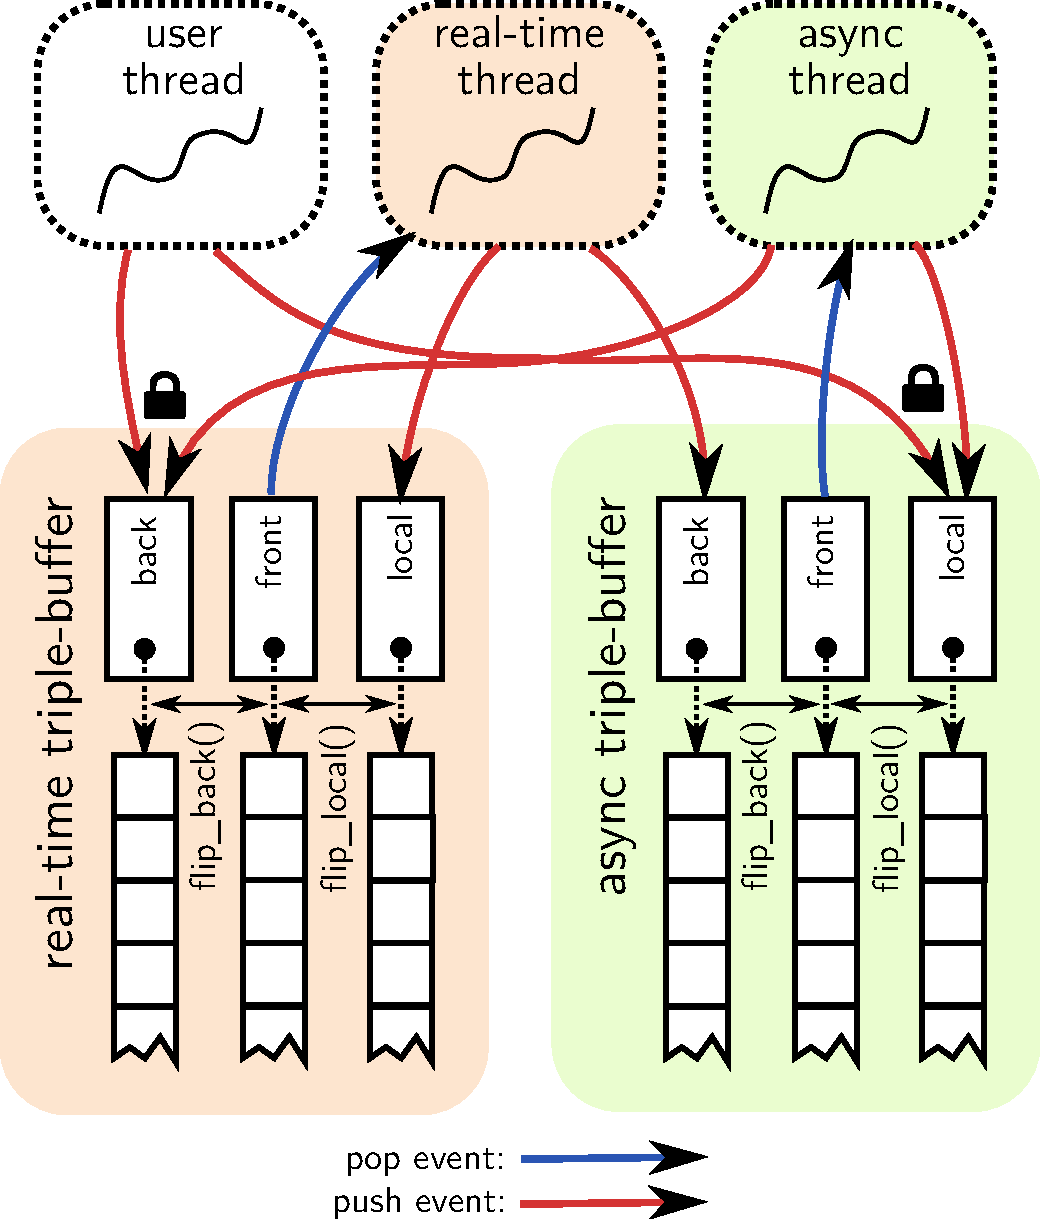
\includegraphics[width=.9\textwidth]{pic/events.pdf}
  \caption{Communication with triple buffer event deques.}
  \label{fig:triplebuf}
\end{figure}

\begin{description}
\item[Front buffer] \index{flip (multiple-buffering)}This is the
  buffer where the events are popped from for processing. Only the RT
  thread should access the front of its triple buffer, and the same
  happens in the async thread.

\item[Back buffer] This is, in general, the buffer where events coming
  from other threads are written to. In the RT triple buffer case, the
  both the user thread and the async thread do write into it, but they
  synchronise their insertions with a mutex --- because they can! The
  \type{flip\_back ()} method exchanges the front and back
  buffers. The flip is done in the RT thread, at the beginning of each
  process request, thus should can not contend for the mutex. Instead
  it does a conditional lock, and if it fails, it skips the flip. This
  may cause some events to be delayed more than one request if there
  is a lot of contention on the mutex --- i.e. the user and async
  threads are writing a lot of events --- but that does not happen in
  practise and informal experiments suggest that the approach is
  enough. However, this could be completely solved by implementing
  lock-free \type{hetero\_deques}, at least lock-free for one writer
  and one reader. We develop this idea in section
  \ref{sec:improvehetero}. In that case, the user and async thread
  would still need to serialise their writes, but the RT can flip and
  read safely without caring about the mutex at all.

  The back of the async triple buffer is slightly different. Here,
  only the RT thread writes, because if the user thread could write on
  it at the same time we would need a lock. Indeed, it is also the RT
  thread who does the flip after filling it, as long as the async
  thread is not still processing the current front buffer, otherwise
  the flip is postponed.

\item[Local buffer] The local buffer is where a buffer writes events
  that he sends to itself. Thanks to this, we can have a notion of
  ``post-processing'' and also infinitely recursive events that
  generate a new event each time. This is very useful for implementing
  \emph{tasks} and state machines. If a thread wrote his own events in
  its front buffers, this kind of behaviour would lead to an infinite
  loop and events sent to the back buffer would never be
  processed. The \type{flip\_local ()} method exchanges the front and
  local buffers.

  Note that in the local buffer of the async thread is a bit
  special. Because the RT thread has exclusive non synchronised access
  to the back buffer, events from the user thread are sent to the
  async thread through the local buffer, and they use a mutex to avoid
  data races.
\end{description}

While this structure might seem a bit baroque, all the complexity is
hidden in the \type{processor} and \type{*\_process\_context}
classes. In most cases, one should only care about making the right
choice of which thread should execute our event; all the dispatching
and processing happens transparently and the type system ensures we
can only do it in a thread safe way --- thanks to the three-tier
processing contexts.

Listing \ref{lst:nodeexample1} shows an example on how to use this
event passing system. The frequency parameter is set from the user
thread, but it must be read from the RT thread and the related
variable \emph{rt\_dt} must be updated. Doing this in a portable and
thread-safe way without using mutexes is tricky. Thanks to our
structure, we just send an event that does the job of updating the
variables. There are no possible data races even if reading/writing
float values is not atomic, because the lambda expression captures a
local copy of the \type{freq} variable. This is a very convenient
fact: the event's own state provides an intermediate buffer for
communicating value updates without data races; the lambda semantics
in C++0x just provides us the syntactic sugar to make the code
pleasant to write and read. Please remember that this code is here
only to illustrate the usage of the event passing system; in practice,
passing parameters from the user thread to the RT thread is even
simpler, as we will explain in the following.


\begin{lstlisting}[float=h!, label=lst:nodeexample1, caption=A thread communication use-case]
struct example_oscillator_node : public node
{
    example_oscillator_node ()
        : _freq (440.0f) , _rt_freq (_freq), _rt_phase (0)
        , _rt_dt (0) // rt_on_context_update will be executed before
                   // the first process so we can set properly this
                   // variable that depends on the frame rate.
    
    void set_frequency (float freq) {
        _freq = freq;
        auto& ctx = process ().context ();
        ctx.push_rt_event (make_event ([=] (rt_process_context& ctx) {
            _rt_freq = freq;
            _rt_dt   = 1 / (freq * ctx.frame_rate ());
        }));
    }

    float frequency () const
    { return _freq; }

protected:
    void rt_on_context_update (rt_process_context& ctx)
    { _rt_dt = 1 / (_rt_freq * ctx.frame_rate ()); }

    void rt_do_process (rt_process_context& ctx) {
        auto frames = ctx.block_size ();
        while (frames --> 0) {
            // We suppose M_PI is defined. The output_sample function
            // does not actually exist, it is just an example.
            output_sample (std::sin (_rt_phase * 2 * M_PI));
            _rt_phase += dt;
        }
    }

    float _freq, _rt_freq;
    float _rt_phase, _rt_dt;
}
\end{lstlisting}

\subsection{Node components}

In the last section we have seen how we can easily build a notion of
\emph{parameter} similar to the one abstracted in the
analysis section on top of the event passing infrastructure. However,
there are a few ways we can criticise the approach in listing
\ref{lst:nodeexample1}:
\begin{enumerate}
\item Even though the code is not too large, in the presence of nodes
  with many parameters we could easily devise a recurring pattern
  calling for a refactoring. Indeed, we always do the same to pass
  information from the user to the node's processing state: store a
  copy for the user and another one for the node's internal processing
  in the RT thread --- to update the later from the user thread, we
  send a RT event. For controls working in the other direction, this
  is, controls intended to send information from the RT thread to the
  user, this is a bit less trivial because it involves sending the
  update through the async thread and, if the status control type does
  not have an atomic assign operation, locking a mutex to avoid data
  races between the user and async thread. It seems reasonable to
  abstract this behaviour and relieve the node implementer from
  rewriting this patterns \emph{ad-nauseum}. Moreover, if abstracted
  as a class, these controls can be later extended by themselves, for
  example, to add polyphonic support.

\item There are some corner cases that the previous code does not
  address. Actually, if the node is not attached to a processor that
  code would throw a \type{node\_attachment\_error} exception when it
  invokes the node's \type{process ()} method inside
  \type{set\_frequency ()}. It does make sense to alter the node
  frequency before attaching it to a process, so this limitation
  should be avoided. Moreover, even if the node is attached but the
  process is not started, events would accumulate in the queue. If the
  node is detached from the processor before the network is run, the
  internal frequency would never be updated indeed. This shows how
  there are many corner cases, and isolating this complexity in a
  class with its own responsibilities yields safer code.

\item Manipulating the frequency parameter as implemented in that code
  requires knowing the node's concrete type. This is a show stopper
  for the \emph{plugin} that we shall implement in the next
  iteration. Instead, parameters should be accessible directly from
  the node's basic interface, and identified with strings, such that
  using them requires no compile-time binding at all.
\end{enumerate}

This results in the notion of \index{component (node)}
\emph{component}: an attribute associated to a node, that may be of
four kinds; an input port, an output port, a input control or an
output control. These four kinds of components have different
properties but there are some commonalities among them too:
\begin{enumerate}
\item They have an unique name (unique within a node and kind of
  component) that identifies them.
\item They have an associated regular type. Regular means that it
  models the \type{Regular} concept, i.e. is default constructible,
  copy-constructible and copyable. This is the type of the data that
  they ``hold'' or ``pass''.
\item They have some associated metadata, which is just a $String
  \rightarrow String$ map providing information that may be useful to
  the user, most of the time to the human user of the application.
\item They can be queried by their name and enumerated from the node
  interface. This is required to allow the implementation of plug-ins.
\end{enumerate}

\subsubsection{Control components}

Figure \ref{fig:controls}\index{control} shows the most important
classes and interfaces implementing the control components ---
i.e. parameter and status variables. \index{parameter (node)}
Parameters or input controls are used to pass information from the
user thread to the node's internal processing state. States or output
controls \index{state (node)} work in the other way, they expose some
internal processing status to the user.

\begin{figure}[t]
  \centering
  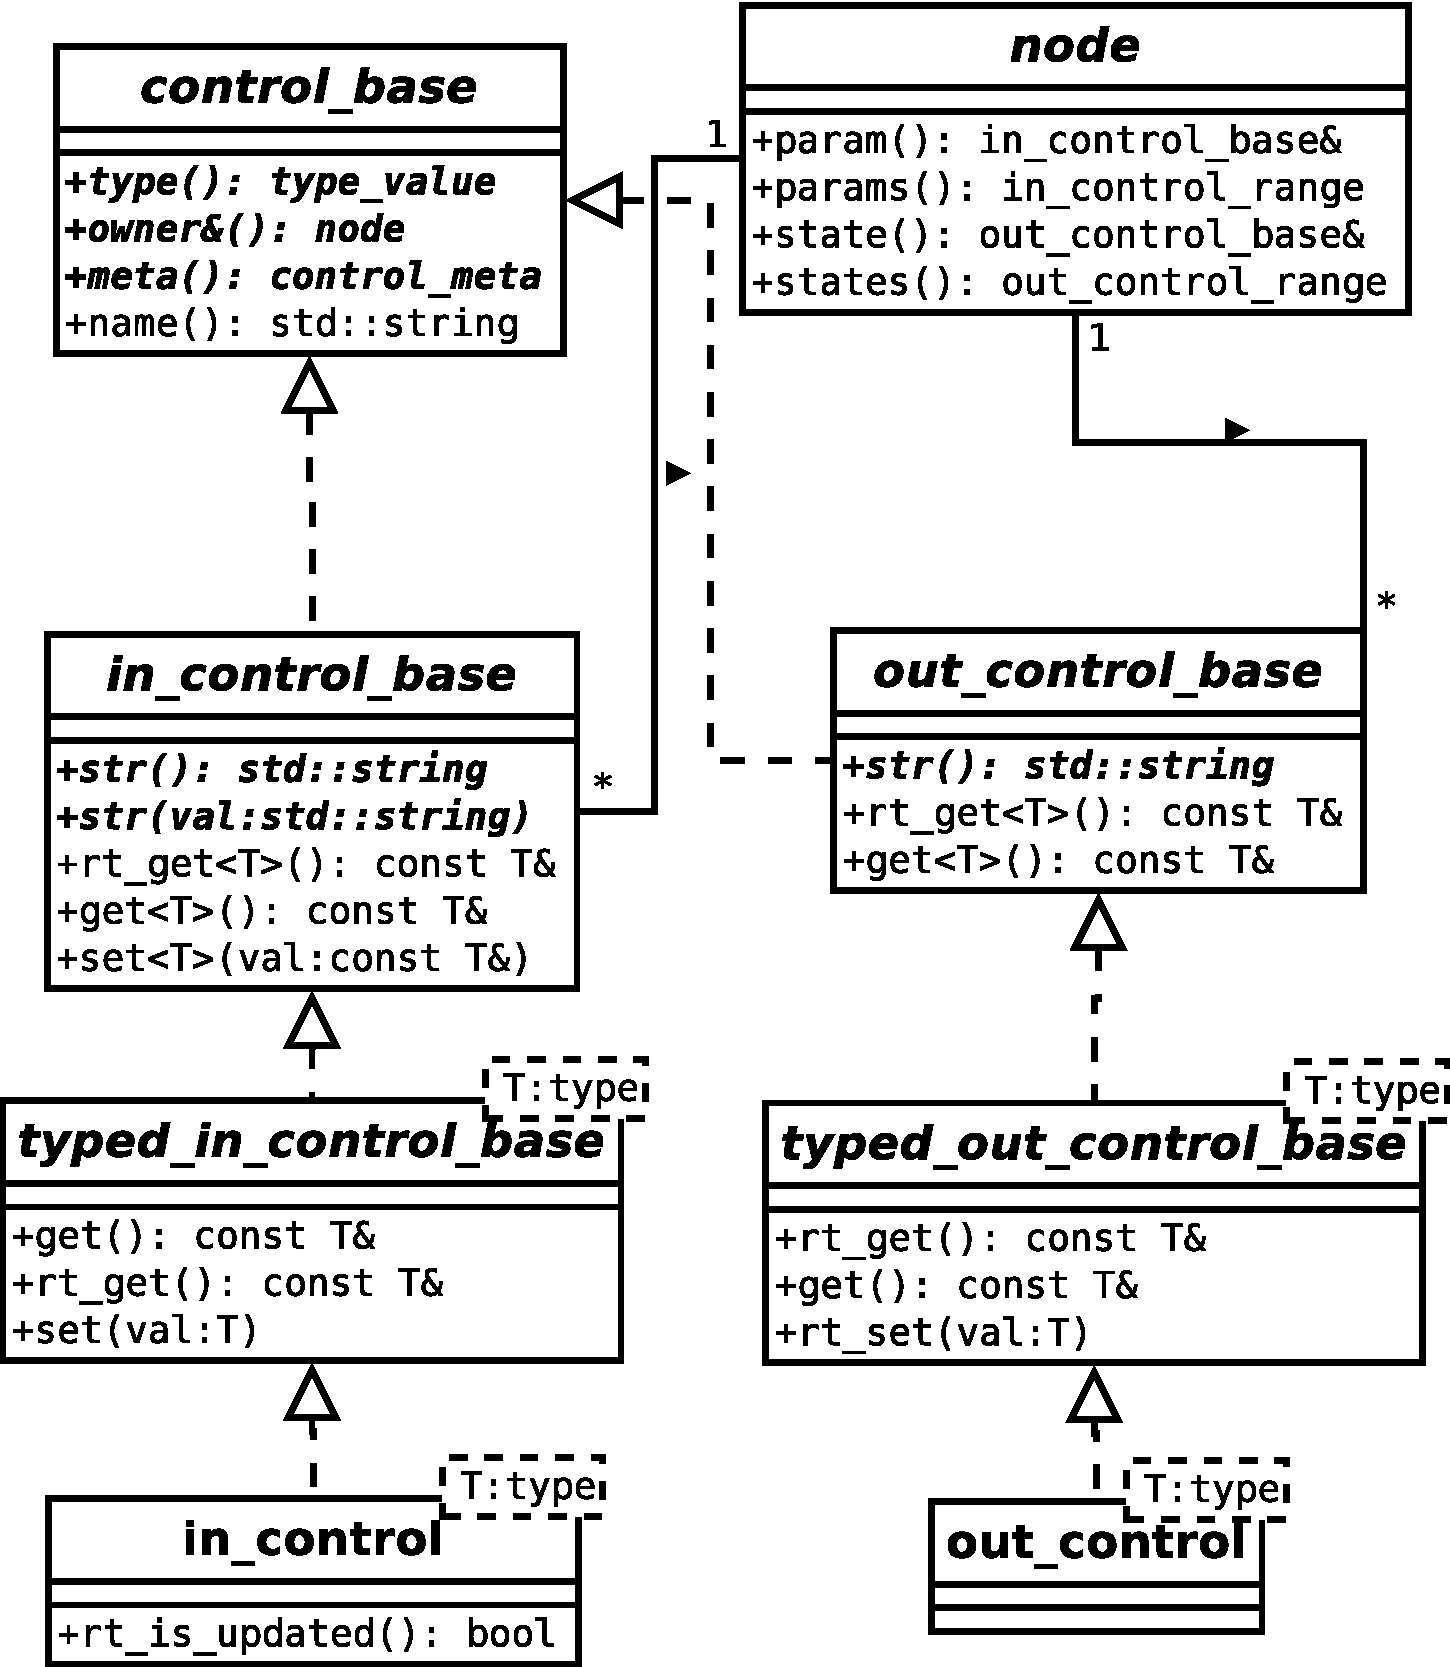
\includegraphics[width=.8\textwidth]{pic/graph-ctl.pdf}
  \caption{UML class diagram of the most important classes for the
    port components.}
\label{fig:controls}
\end{figure}

Note that in the current implementation there is some special
requirement that somehow couples the control bases and their typed
version. If you access the control through the control base access
template method with a type \type{T}, and for that control \type{type
  ()} method returns \type{typeid (T)}, then that object must be a
typed control of type $T$; otherwise this is undefined behaviour. In
practice, this means that you must never inherit from
\type{in\_control\_base} or \type{out\_control\_base} directly, but
you should inherit from their typed versions instead.

\subsection{Port components}
\label{sec:modports}

\begin{figure}[t]
  \centering
  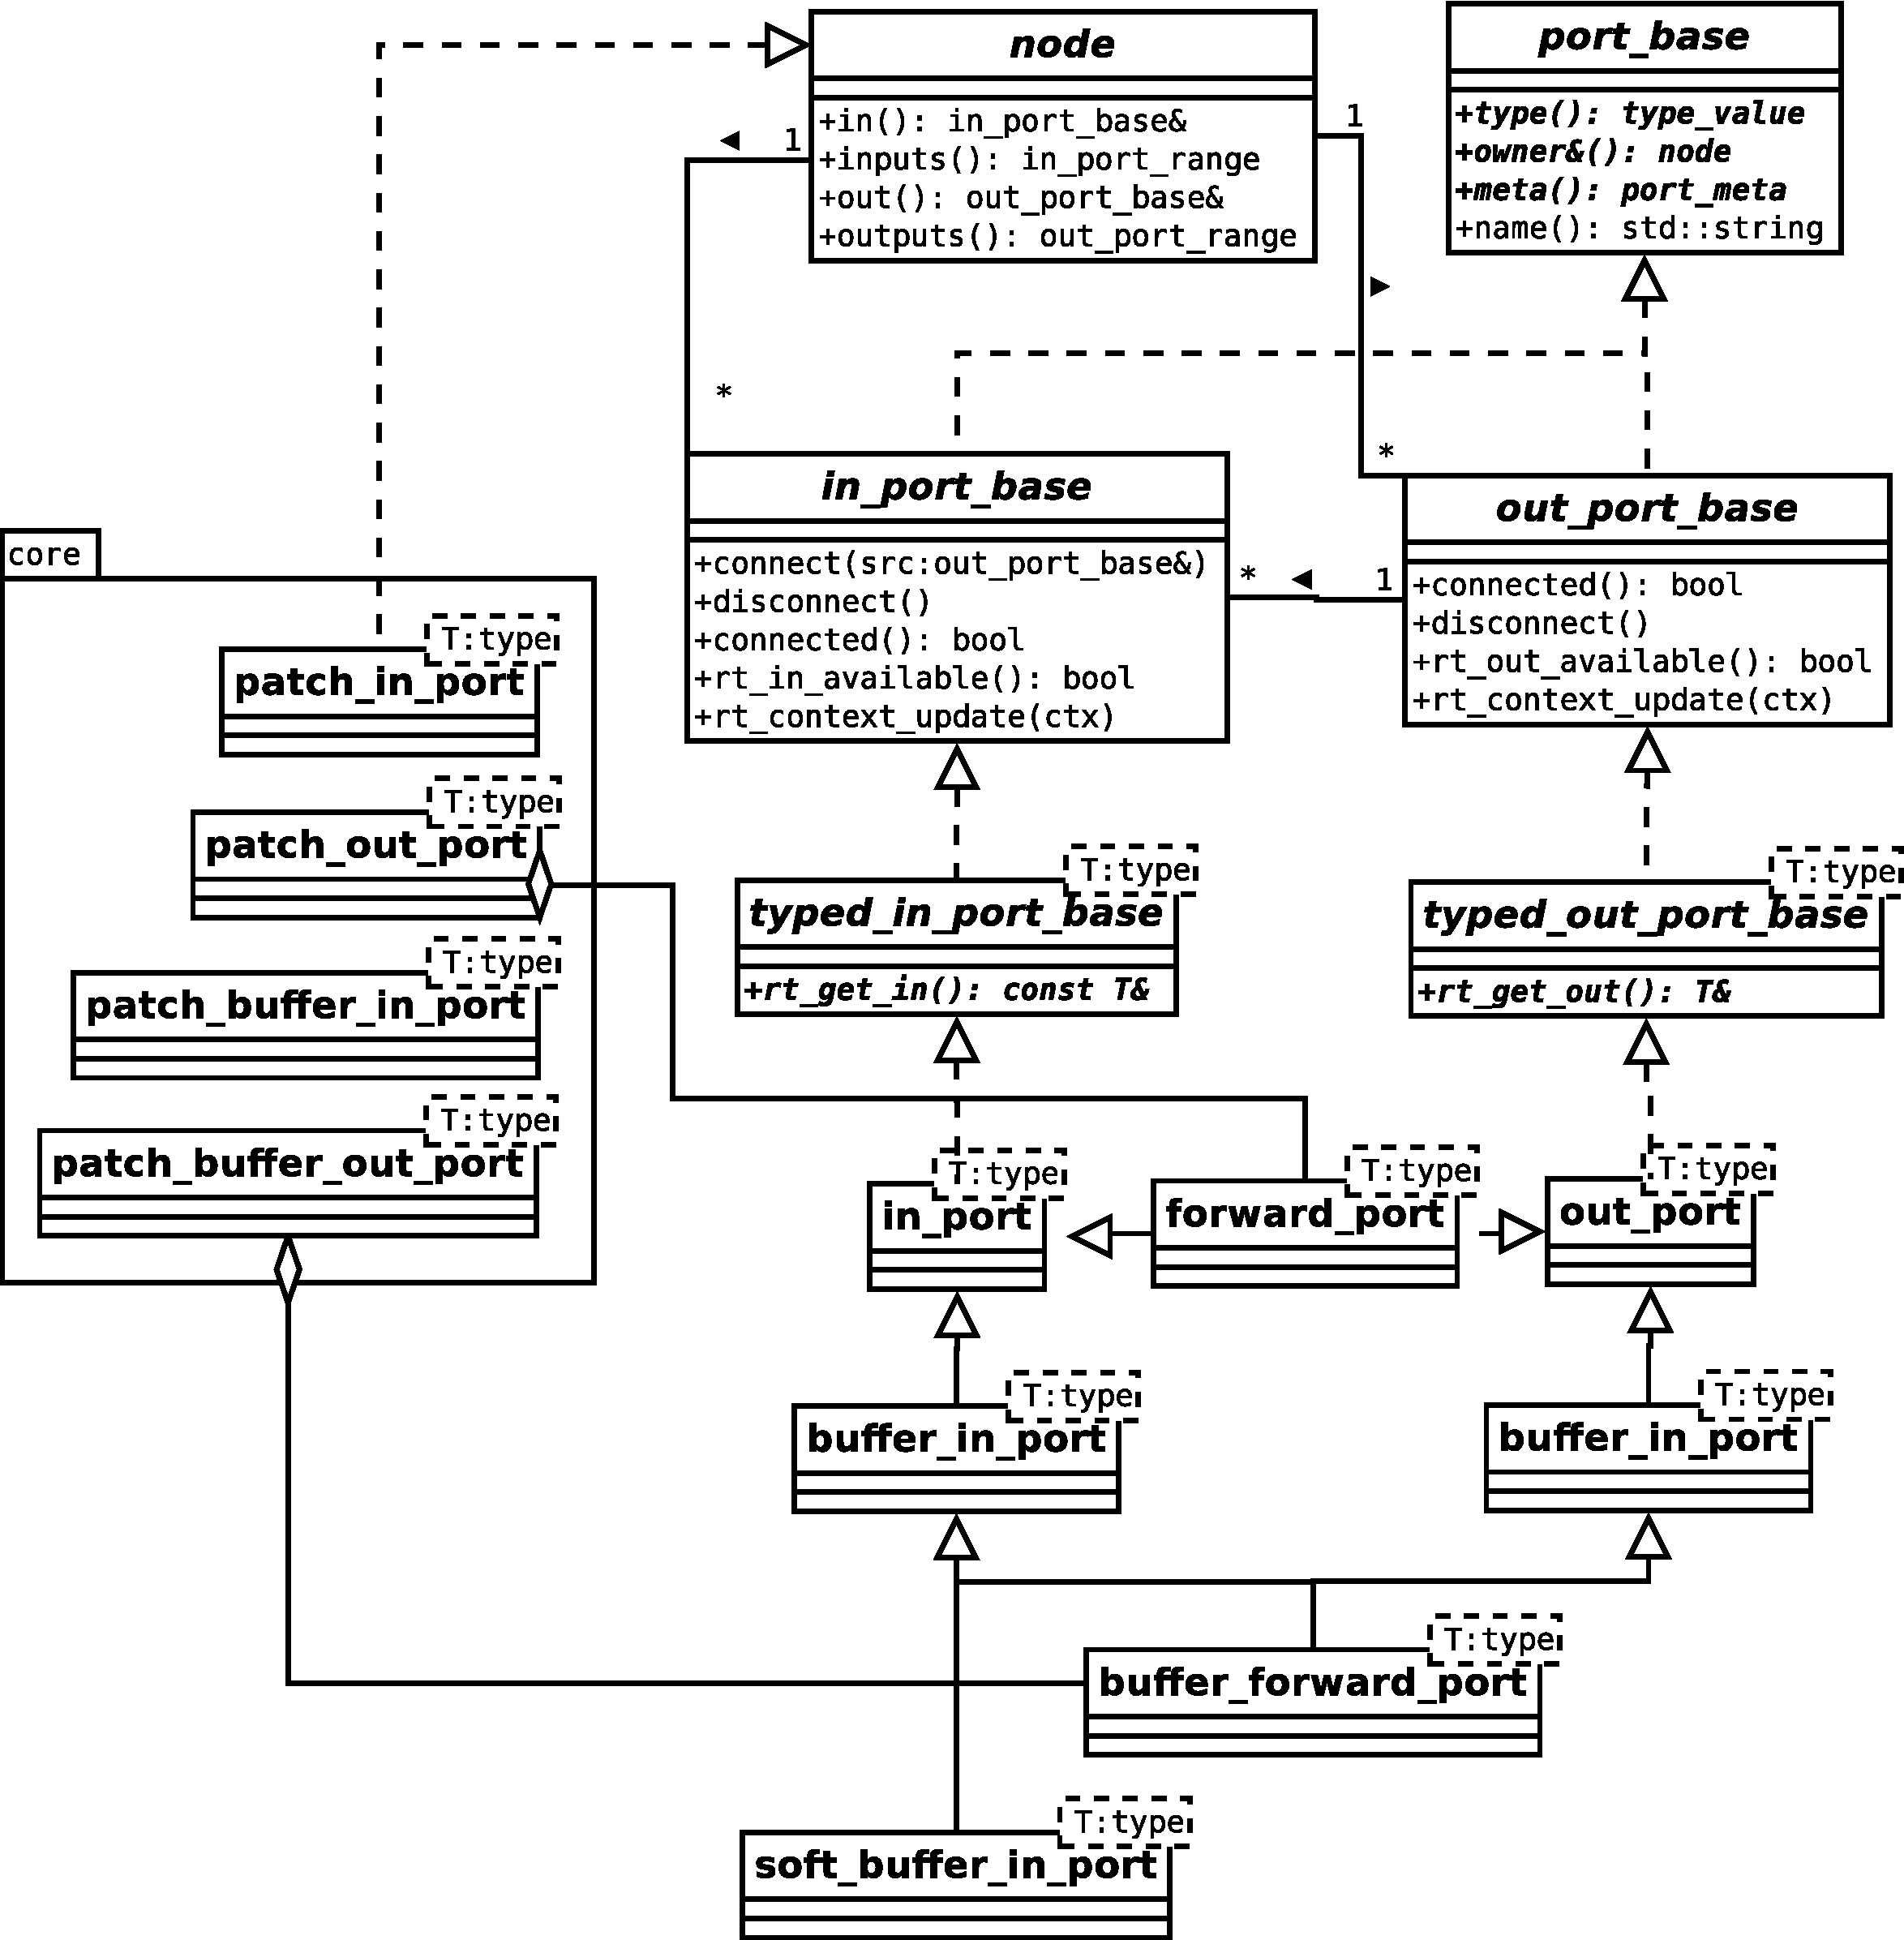
\includegraphics[width=\textwidth]{pic/graph-port.pdf}
  \caption{UML class diagram of most important classes for the
  control components.}
\label{fig:ports}
\end{figure}

Figure \ref{fig:ports} shows the most relevant classes implementing
the notion of \emph{ports}\index{port}. There are two symmetric kinds
of ports, input and output. Following the analysis in the first
section, these ports are related in a one-to-many manner --- an output
port may be connected to many input ports. These ports thus give the
graph shape to patches. As we can see in the diagram, concrete ports
are parametrised over the signal type but a polymorphic interface
exists providing its basic functionality. While this diagram is very
similar to that describing the \emph{controls} in figure
\ref{fig:controls}, ports have some added complexity and there are
some extra classes that are worth mentioning.

First, we have to distinguish between audio-rate and control-rate
signals. Usually, we store audio-rate signals in sound buffers
modelling the \type{BufferConcept} we developed in the previous
chapter. These buffers should be able to allocate a whole bunch of
\type{block\_size} frames; to enforce this invariant, some mechanism
should react on process context update notifications to ensure that
the buffer size matches the current processing block size. The
\type{buffer\_out\_port} and \type{buffer\_in\_port} do this
transparently to the user, but they impose a \type{BufferConcept}
requirement on their type parameter $T$. For control rate signals,
using a simple \type{in\_port} or \type{out\_port} suffices.

Another important issue that we have to address is: how do we add
ports to a patch node? Note that the relation between components and
nodes is somewhat static --- actually the port or control constructor
takes care of establishing the relationship. We should expect that,
like in most modular synthesis software, the user can arbitrarily
manipulate which ports are exposed from within a patch. The most
natural way of manipulating a patch is by manipulating nodes, thus,
ports are exposed by special kinds of concrete nodes like the ones in
the \type{core} package in the diagram. The \type{patch} class detects
whenever a port node is added and exposes it in its interface. A
``patch input port node'' would show as an input port in the patch
that contains it, and the \emph{``port-name''} parameter of the node
controls the name that the port has in the patch interface. The port
node itself has an output port, that can be connected to any other
node within the patch. A ``patch output port node'' works in the
opposite way: it exposes an output port externally and an input port
internally. These kind of nodes are implemented using the
\index{forwarding prot}\emph{forwarding ports}, which allow
implementing a sort of \emph{identity function} node without the
overhead of copying the input into the output. When its output is
requested, they just return a reference to its input data.

More problems arise when we consider that ports may be disconnected
and reconnected at any point in time, a precondition for the high
interactivity that we want to achieve with our system. As a matter of
bad luck, it may happen that we disconnect a port just when the
incoming sound signal is at a ``high'' value. Figure
\ref{fig:soft-port-0} (a) represents the actual signal that is going
through an hypothetical input port which is connected to a sinusoid
generator and then suddenly disconnected. If this signal is emitted to
the speakers, we would hear a very disruptive ``click'' noise at the
point of disconnection because an instantaneous change can be consider
of infinite frequency that the DAC in your sound card will just mess
up.

\begin{figure}[t]
  \centering 

  \subfloat[A click is produced on a
  disconnect.]{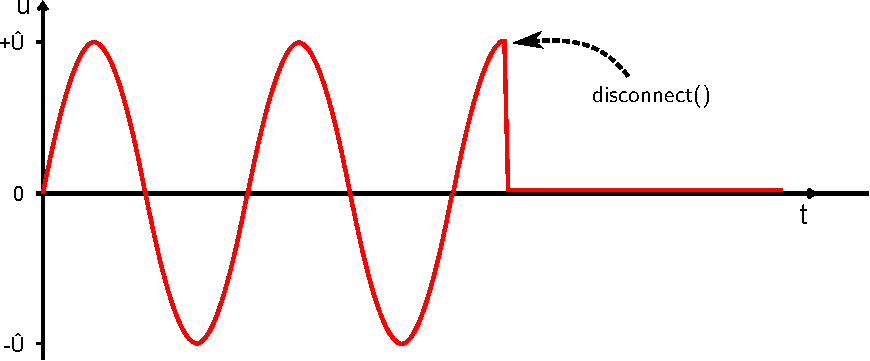
\includegraphics[width=.8\textwidth]{pic/soft-port-0.pdf}}
  
  \subfloat[Solution by delaying the actual disconnection and
  enveloping the
  signal.]{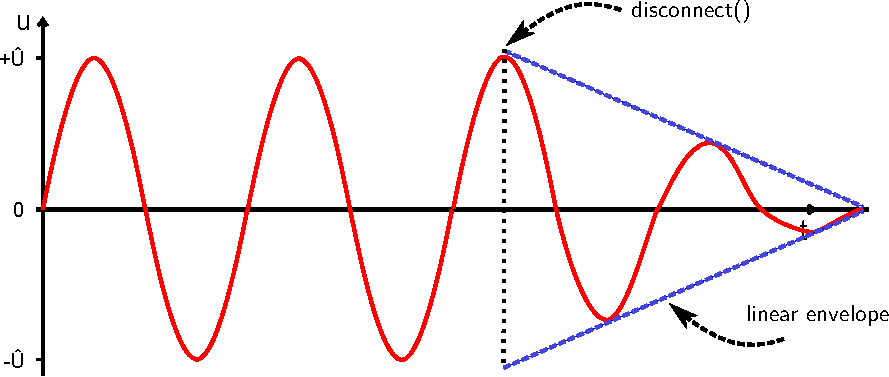
\includegraphics[width=.8\textwidth]{pic/soft-port-1.pdf}}
  \caption{The problem of softening a signal disconnection.}
\label{fig:soft-port-0}
\end{figure}

There are few ways to solve this problem. For example, the Audacity
\footnote{\url{http://audacity.sourceforge.net/}} sound editor
automatically modifies selection edges on the sound wave slightly to the
closest positive-slope zero crossing when the \emph{Find Zero
  Crossings} option is enabled. In a similar way, we could delay a
disconnection until the signal goes back naturally to zero.

While we might implement that behaviour in the future to make it
optionally available when it makes sense, we have implemented a bit
more general solution that works sufficiently well even with LFO's
where the former approach would introduce too much latency. Instead of
waiting for the source signal to go back to zero, we directly apply a
linear envelope that goes from 1 to 0 and only wait for the envelope
to reach the 0. Figure \ref{fig:soft-port-0} (b) illustrates this
effect. The length of the envelope is fixed and thus the latency
introduced by the anti-click mechanism is deterministic and we can
keep it as small as we want. The length of the envelope defaults to a
conservative value of $4 ms$. The reasoning behind this is that in the
worst case it would introduce a slope from 1 to 0 of length $4ms$,
which if it were a signal by itself would have a dominant frequency of
$\sim 50 hz$ that lies around the low threshold that human hearing can
perceive \cite{goldstein01sensation}. The actual artifacts that this
mechanism may introduce in the general case are hard to analyse
formally, but subjective experiments show that it introduces no
noticeable defects on its own and eliminates the click artifact that
we wanted to avoid. The \type{soft\_in\_port} implements this
behaviour and the client can set the envelope length and the stable
value --- whether the signal should fade out to 0, 1 or some other
value --- to adapt this mechanism taking the actual nature of the
expected input into account.

Note that the envelope must be applied both on disconnection and
connection, otherwise a disastrous situation like the one in figure
\ref{fig:soft-port-1} (a) may occur. There, at the marked point in
time the input port of the red signal is disconnected, but the same
signal is connected back into a second port, represented in green. A
dotted blue line show the sum of both the old port that is fading out
and the new port. First of all, the click appears again at the new
input end. Even worse, the total amplitude is unexpectedly big ---
maybe even introducing clipping\index{clipping} --- during the input
signal fadeout. If we apply a rising envelope when a new connection is
made with the same properties that we described previously, the result
is more close to what the user would usually expect, as shown in
\ref{fig:soft-port-1} (b).

In the future we may change the linear envelope with an exponential
envelope, which is suggested to have a better perceived accuracy
\cite{boulanger10audio}. Also, it seems reasonable to use the second
half of a Hann window\footnote{Like the one used to slice a signal
  when applying the Short-time Fourier transform.} as envelope, as it
is designed to produce minimal aliasing \cite{blackman59measurement}.

\begin{figure}[t]
  \centering 

  \subfloat[A click and a power artifact is introduced because of
  coupling a disconnection and a new
  connection.]{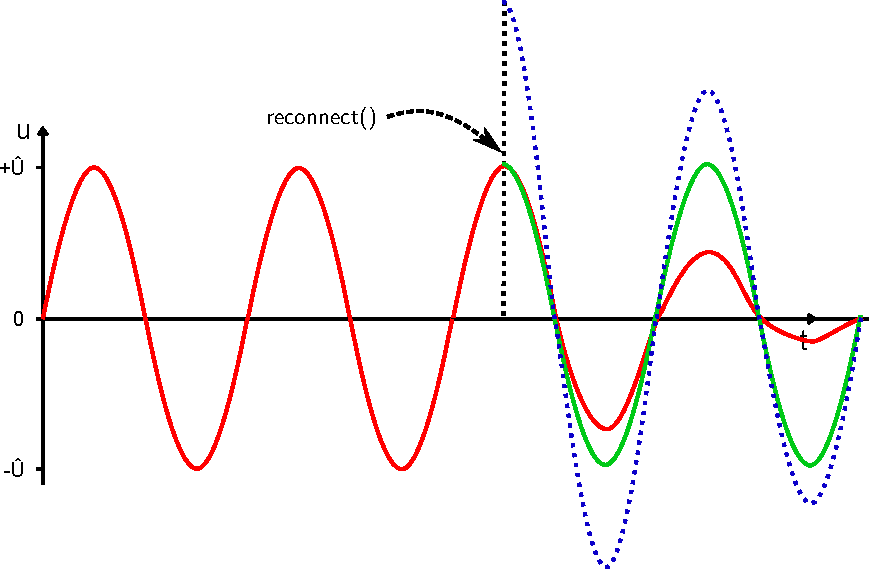
\includegraphics[width=.8\textwidth]{pic/soft-port-2.pdf}}
  
  \subfloat[Solution by enveloping the new
  connection.]{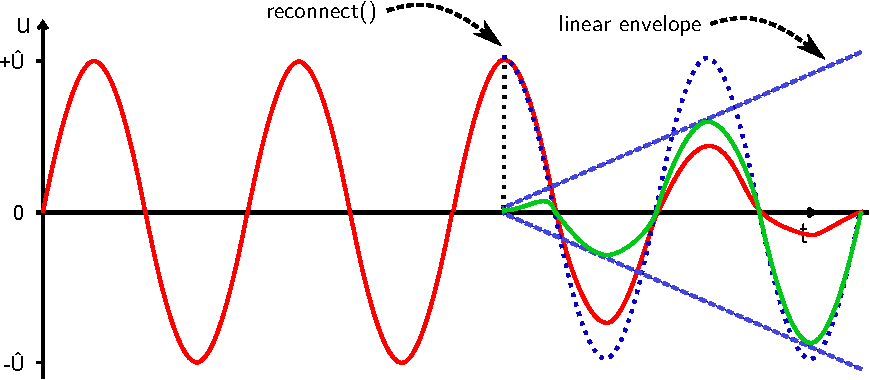
\includegraphics[width=.8\textwidth]{pic/soft-port-3.pdf}}
  \caption{The problem of softening a signal connection.}
\label{fig:soft-port-1}
\end{figure}

\subsubsection{The oscillator node example revisited}

\begin{lstlisting}[float=h!,caption=The oscillator node implemented
  using components,label=lst:nodeexample2]
struct better_example_oscillator_node : public node
{
    buffer_out_port<mono32sf_buffer> out_output;
    soft_in_port<mono32sf_buffer>    in_modulator;
    
    in_control<float> param_frequency;
    in_control<float> param_amplitude;

    better_example_oscillator_node ()
        : out_output ("output", this)
        , in_modulator ("modulator", this, 1.0f)
        , param_frequency ("frequency", this, 440.0f)
        , param_amplitude ("amplitude", this, 1.0f) {}

protected:
    void rt_do_process (rt_process_context& ctx)
    {
        _osc.set_frequency (param_frequency.rt_get ());
        _osc.set_amplitude (param_amplitude.rt_get ());
        _osc.update_fm (out_output.rt_out_range (),
                        in_modulator.rt_in_range ());
    }

    void rt_on_context_update (rt_process_context& ctx)
    { _osc.set_frame_rate (ctx.frame_rate ()); }

    synth::oscillator<synth::sine_generator> _osc;
};
\end{lstlisting}

We are now ready to devise a more realistic implementation of the
oscillator node that we introduced in listing
\ref{lst:nodeexample1}. The new code in listing \ref{lst:nodeexample2}
shows that by using the new constructs that we built in this section,
not only is the code safer and more extensible and featured, it is
also clearer and more concise. This code introduces the
\type{synth::oscillator} class (section \ref{sec:ns-synth}). Also,
this oscillator allows frequency-modulation, this is, to vary the
oscillator frequency using an optional input signal. We do not need to
check whether the optional modulator is connected, because an input
port with softening defaults to its \emph{stable value} when it is
not connected.

\subsection{Indirect object construction}
\label{sec:graphfactory}

\index{factory (design pattern)}In the presence of plug-ins, the main
control flow of the program never gets to know at all the concrete
type of some objects, and they are used only through its abstract
interface. Even without plug-ins, it is quite convenient when writing
a user interface to be able to choose the concrete type of an object
dynamically --- identified by a run-time value like a integer or a
string. The \emph{factory method} and \emph{abstract factory} design
patterns coordinate to provide this feature \cite{gamma95design,
  vlissides98pattern}.

\index{singleton (design pattern)}We wrote the pattern as a set of
reusable template classes, following ``Modern C++ Design''s advice
\cite{alexandrescu01modern}. We extended his implementation with
improved safety when using smart pointers, decoupled abstract
factories and methods, and customisable constructor signatures. Many
times factories make more sense as \emph{singletons}, and some of our
factories --- \emph{restricted static factories} --- can only be
instantiated as a singleton.  The \type{base::singleton\_holder<T,
  CreationPolicy, Lifetime\-Policy, Threading\-Policy>} may be used
build a singleton type from any type $T$, offering control over the
life-time of the object, its construction and the thread safety of the
singleton access method. The interested reader can read the attached
source code or the reference manual for further information on these
classes.

A singleton factory manager for creating nodes is defined as:
\begin{lstlisting}
typedef 
base::restricted_global_factory_manager<std::string, node_ptr>
node_factory;
\end{lstlisting}

The \type{self ()} method returns the singleton instance and then the
\type{create (std::string id)} method returns a new instance wrapped
in a safe shared pointer \type{node\_ptr} --- remember that this is an
alias for \type{std::shared\_ptr<node>}. Creating a new instance thus
does not require including the header that declares the concrete type,
and it can be chosen based on a value determined by external
input. For example, we can create an oscillator as simply as in:
\begin{lstlisting}
    node_ptr osc = node_factory::self ().create ("audio_sine_oscillator");
\end{lstlisting}

New types can be registered in the factory only by instantiating an
instance of the \type{node\_factory::registrant<T>} type and its
constructor takes the name that should identify the type. This is so
because it is a \emph{restricted} factory, other kinds of factories
have a \type{add ()} and \type{remove ()} methods for registering
types at any time. This restricted singleton factory enforces doing
the registration of the types before the \type{main ()} function
starts by instantiating the registrant as a global variable. The
following macros ease this common pattern of use:

\begin{lstlisting}
#define PSYNTH_REGISTER_NODE_STATIC(node_type) \
    static ::psynth::graph::node_factory::registrant<node_type> \
    node_type ## _registrant_ (#node_type);

#define PSYNTH_REGISTER_NODE_STATIC_AS(node_type, node_name) \
    static ::psynth::graph::node_factory::registrant<node_type> \
    node_type ## _registrant_ (node_name);
\end{lstlisting}

To register the node that we defined in listing
\ref{lst:nodeexample2}, we would write in its \type{.cpp}
implementation file at global or namespace scope:
\begin{lstlisting}
  PSYNTH_REGISTER_NODE_STATIC(better_example_oscillator_node);
\end{lstlisting}

This mechanism can be used as a primitive plug-in system. If we open a
shared library file (e.g a \type{.so} file in GNU/Linux) using the
Unix \type{dlopen ()} function it would automatically instantiate any
global registrant and we could already create any object provided by
the plug-in passing their name as a string to the factory. Indeed,
some authors propose this mechanism for dynamic loading of C++ classes
\cite{norton00dynamic, beveridge98self}. However, a practical plug-in
system must be a bit more sophisticated to do proper versioning, ease
metadata access and put the main program --- and not the plug-in ---
into control of the registration\footnote{In these slides we discuss
  the tricky corners of implementing a plug-in system in C; a lot of
  what it states applies to C++:
\url{http://colinaroja.org/files/charla_c.pdf}}.

\subsection{Going Model-View-Controller}
\label{sec:graphmvc}

So far, we have concentrated on devising the core of the audio
processing engine. At some point, we will need to write user
interfaces --- indeed, we already have written a 3D experimental user
interface and a command line user interface that can inter-operate
over the network, and we have plans to build a custom user interface
for tangible devices and another one for multi-touch pads. These user
interfaces deserve a whole project on their own; as our main
objective states (section \ref{sec:mainobjective}), we shall
concentrate on the basic framework \emph{enabling} and supporting the
rapid development of these interfaces. For this purpose, requirement
\ref{req:views} suggests that we provide the hooks to independently
write collaborating views.

\index{MVC, model-view-controller}The Model-View-Controller, which is
often regarded as an architecture, sometimes a pattern, or in its
original paper as \emph{paradigm} \cite{krasner88mvc}, provides the
basic structure that we shall implement to satisfy requirement
\ref{req:views}. When decoupling a system into a MVC arquitecture,
there is this simple guideline, quoted in a software arquitects wiki
as \emph{the best rubric
  ever}:\footnote{\url{http://c2.com/cgi/wiki?ModelViewController}}
\begin{quote}
  ``We need \emph{smart} models, \emph{thin} controllers, and
  \emph{dumb} views''
\end{quote}
This translates in our system as the following:

\begin{description}
\item[Model] \index{model (MVC)}The core of our model is the synthesis
  network, this is, a \type{patch} and related classes. These classes
  maintain the invariants and do the work of processing the sound.

  However, the \type{patch} class is not suitable as a model by
  itself. One of the main properties of a model is that it should be
  \emph{observable}. This means that it should use some
  \emph{inversion of control} mechanism to notify the views on any
  externally visible change of its state. This is usually an instance
  of the \emph{observer} design pattern \cite{gamma95design,
    vlissides98pattern}.\index{observer (design pattern)} A separate
  set of classes wrap the \type{psynth::graph} layer providing this
  observable interface --- we call this the \type{psynth::world}
  layer, that should be renamed in the next iteration as the
  \type{psynth::model} layer. Figure \ref{fig:world} gives an overview
  of this layer. Observability is decoupled from the graph layer
  itself because (1) we get an extra design indirection that allows
  more API flexibility during the fast development of the graph layer
  and (2) avoids the sometimes significant overhead and bookkeeping
  that the observable interface requires, thus enabling the usage of
  the graph layer in isolation where no flexible UI's are required ---
  e.g. in embedded systems or integrated in some other third party
  system.

\item[Views] Views react to the model events producing, usually,
  visible side-effects in the real-world. Note that this notion of
  view is abstract and does not necessarily imply producing a visual
  representation of the model. An example of such non-visual view is
  the component that sends network events in reaction to local changes
  to keep remote synthesisers synchronised. The \type{psynth::net}
  namespace contains the views and controllers required for network
  synchronisation, using the \index{OSC, open sound control} OSC
  protocol \cite{center03osc}. Another example of view maintains a 3D
  visual representation of the synthesis state and is implemented in
  the \type{gui3d} module.

\item[Controllers] Controllers are usually what glues views and models
  together. They are usually do not require any special pattern or
  indirection; controllers are the set of objects that invoke mutating
  actions on the model. Because the observer pattern is used to notify
  the views, controller-view pairs are completely independent of
  each-other and each should work properly regardless or whatever
  views or controllers are also registered in the model. This clearly
  simplifies the implementation of a user interface or a network
  synchronisation system in a completely orthogonal and optional
  manner.
\end{description}
\begin{figure}[h!]
  \centering
  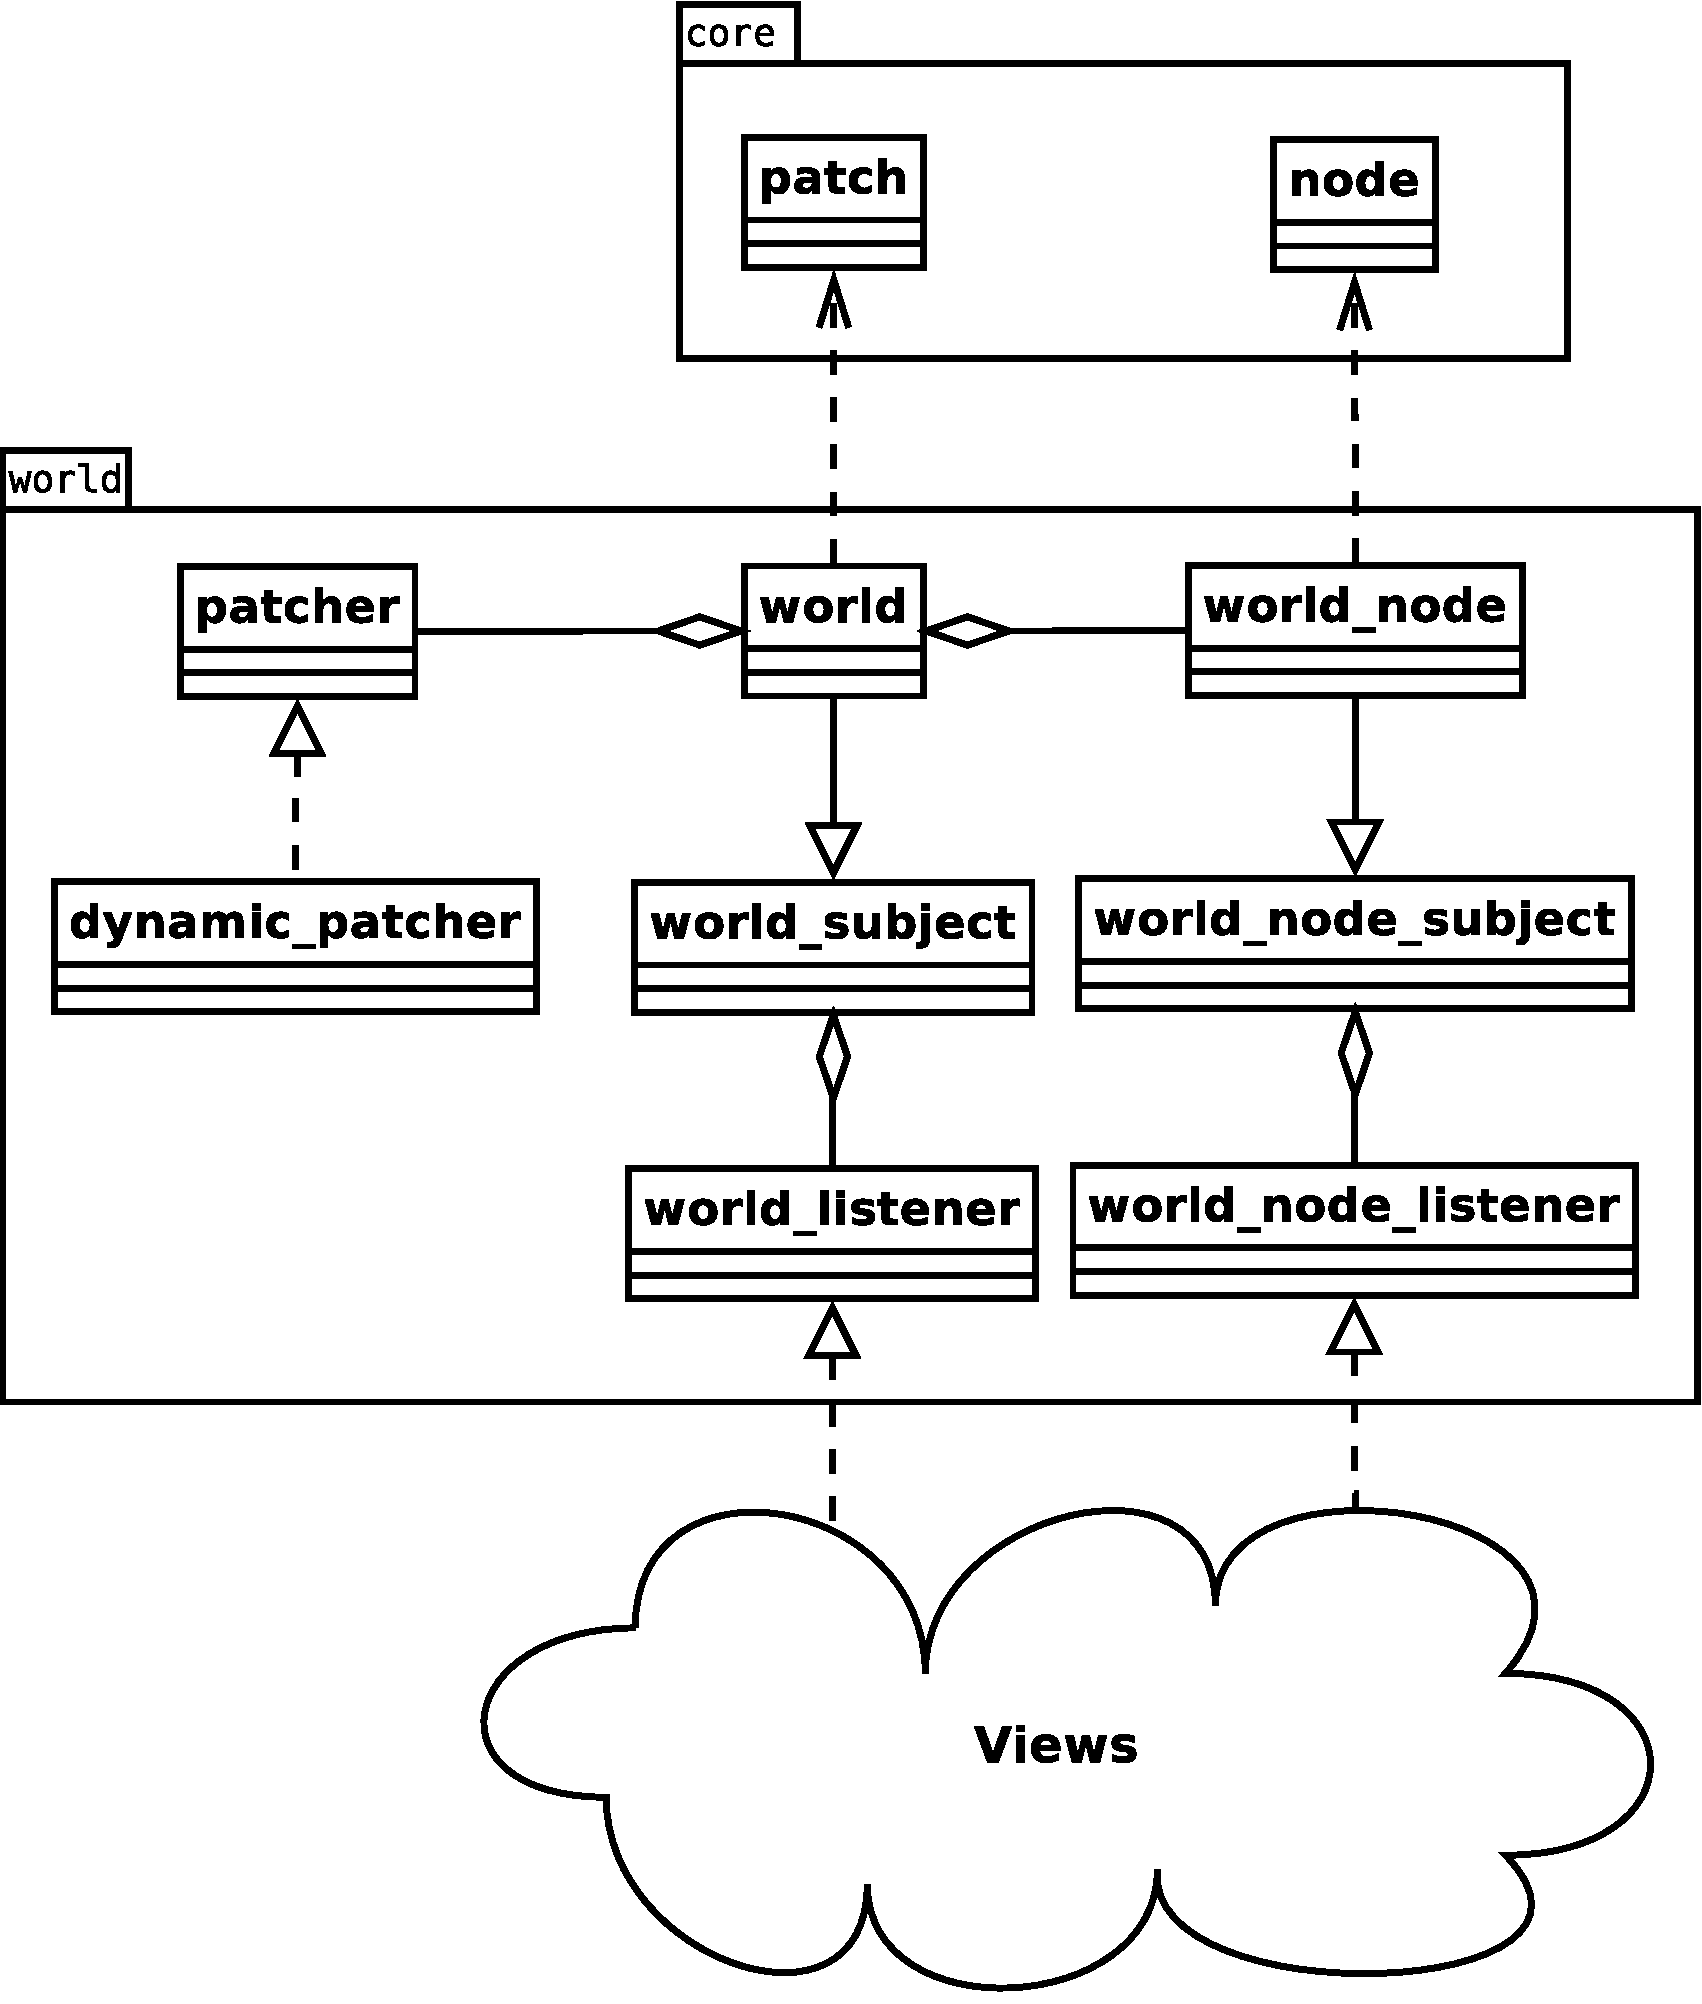
\includegraphics[width=\textwidth]{pic/world.pdf}
  \caption{UML class diagram of the \type{world} layer.}
  \label{fig:world}
\end{figure}

As we explain in section \ref{sec:graph-integration}, integration
of the new graph layer in the rest of the system has not been done
already. This means that the work of modifying the \emph{world layer}
to use the new system is yet to be accomplished. Because the views and
controllers \emph{never} use the graph layer API directly, but they
call the methods provided by the \type{world} and related classes
instead, once this is done the current user interfaces and networking
modules would require no modification.

The world layer hides directly manipulating the synthesis graph in its
public API and delegates the topology management to a \type{patcher}
derivative. \index{strategy (design pattern)}This implements the
\emph{strategy} design pattern, because the \emph{patcher} can be of
different kinds --- e.g. dynamic, manual, etc. The \emph{dynamic
  patcher} arranges the network such that closest compatible
connections are established.

%% Esta descripción es muy formal y queda bonita pero tiene fallos!!!!!
%
% Let $I$ and $O$ be the set of all input and output ports of all nodes
% in a patch, we can define the graph $G = (V, E)$ where the vertex set
% is $V = I \cup O$, and the edges is $E = \{ (i, o) \mid i \in I \land
% o \in O \land type(i) = type(o) \land node (i) \neq node (o) \}$ that
% contains all the possible connections in the graph. Let $distance (a,
% b)$ be a function that maps two ports to the physical distance in
% their visual representation, the dynamic patcher produces a subgraph
% determined by:
% \begin{align*}E' = \{  (i, o) \mid & (i, o) \in E, \\
% & \forall i'. (i', o) \in E' \Rightarrow i' = i, \\
% & \forall o'. (i, o') \in E' \Rightarrow i = o', \\
% & \forall i'. (i', o) \in E \Rightarrow distance (i', o) \geq
% distance (i, o) \lor \exists o'. (i', o') \in E', \\
% & \not \exists (i', o') \in E'. node (o') = node (i) \land node (i') =
% node (o)
% \}
% \end{align*}

The graph is connected constraining port connectivity in a one-to-one
fashion using distance as criterion to choose connections among the
possibilities, and it also avoids cycles. The resulting graph looks a
lot like the \index{MST, minimum spanning tree}\emph{minimum spanning
  tree} of the graph constructed by nodes and all possible connections
and edges weighted on the spatial distance of the interconnecting
nodes in the visual representation. In fact the problem is almost an
instance of the dynamic MST problem \cite{spira75dmst} which can
handle fast a recomputation of the MST when a small update of the
input data happens --- e.g. the weight of one edge changes, for
example, when moving an node.

The main impediment to trivially adapt the world layer to use the new
graph layer is the \emph{dynamic patcher}, because it uses a matrix
based on static information about all possible nodes to check whether
two ports are compatible. This static information is no longer
available and dynamic metadata is provided instead to ease
implementing a plug-in system, as we long discussed in this
chapter. We will delay adapting the dynamic patcher until the plug-in
system is fully implemented in order to avoid rewriting it in the
presence of unexpected API changes.

\todo{Añadir las cosas que había pensado ya sobre los plugins}

\section{Validation}

\subsection{Unit testing}
\label{sec:sound-unittest}

Most of the reasoning favouring the implementation of unit tests in
section \ref{sec:sound-unittest} applies here. Note
\ref{note:graph-test} shows a briefing of the test suite results for
the modules described in this chapter. Note that some suites in the
\type{base} layer that were developed as support for this module are
resented there too --- like, for example, generic singletons,
factories and heterogeneous deques. A total of 206 assertions are
checked in 54 unit tests.

\begin{mynote}[\texttt{psynth::graph} and some \texttt{psynth::base}
  unit tests]
\label{note:graph-test}
The user can run the unit tests by herself by running \texttt{make
  check} or running the \texttt{psynth\_unit\_tests} in the
\texttt{src/test} folder. This kind of report may be generated passing
the \verb|--report=detailed| parameter when running the test script
directly.  {\small
\begin{verbatim}
Test suite "c3_class_test_suite" passed with:
  10 assertions out of 10 passed
  10 test cases out of 10 passed

Test suite "base_exception_test_suite" passed with:
  16 assertions out of 16 passed
  4 test cases out of 4 passed

Test suite "base_hetero_deque_test_suite" passed with:
  87 assertions out of 87 passed
  9 test cases out of 9 passed

Test suite "base_factory_test_suite" passed with:
  8 assertions out of 8 passed
  4 test cases out of 4 passed

Test suite "graph_processor_test_suite" passed with:
  23 assertions out of 23 passed
  9 test cases out of 9 passed

Test suite "graph_core_test_suite" passed with:
  1 assertion out of 1 passed
  1 test case out of 1 passed

Test suite "graph_port_test_suite" passed with:
  1 assertion out of 1 passed
  1 test case out of 1 passed

Test suite "graph_control_test_suite" passed with:
  36 assertions out of 36 passed
  12 test cases out of 12 passed

Test suite "graph_patch_test_suite" passed with:
  24 assertions out of 24 passed
  4 test cases out of 4 passed
\end{verbatim}
}
\end{mynote}

\subsection{Performance}

Quoting Donal Knuth is the best way to illustrate current trends
towards software optimisation \cite{knuth74structured}:
\begin{quote}
  \it Premature optimisation is the root of all evil.
\end{quote}

The reasoning behind this phrase is that micro-optimising every single
part of our code is futile. It does not lead to faster programs,
instead, doing so increases the complexity of the code, leading to
subtle bugs and making harder, if not impossible, to later redesign
the code to implement better algorithms that would give a much larger
performance boost. A much better methodology suggests to concentrate
on program correctness. When the program has been validated,
\index{profiling}\emph{profiling} provides a way to detect,
empirically, what parts of the program are consuming most time. Then,
if needed, we can optimise the slow parts, which usually are deep in
the call graph, just inside the most nested loops.

We developed a program that, we believe, is a good stress test for our
system and executes most relevant code paths of our system. This
program runs the synthesis graph in figure \ref{fig:perfgraph} for 10
seconds. Note that dashed lines represent patches and big black dots
are patch ports. The other spheres are other kinds of nodes. The
following events are generated during the execution:
\begin{itemize}
\item Every $0.1 s$ it randomly changes the value of all the
  oscillators.
\item Every second it randomly connects or disconnects the links
  between modulators and generators.  
\end{itemize}

\begin{figure}[h]
  \centering
  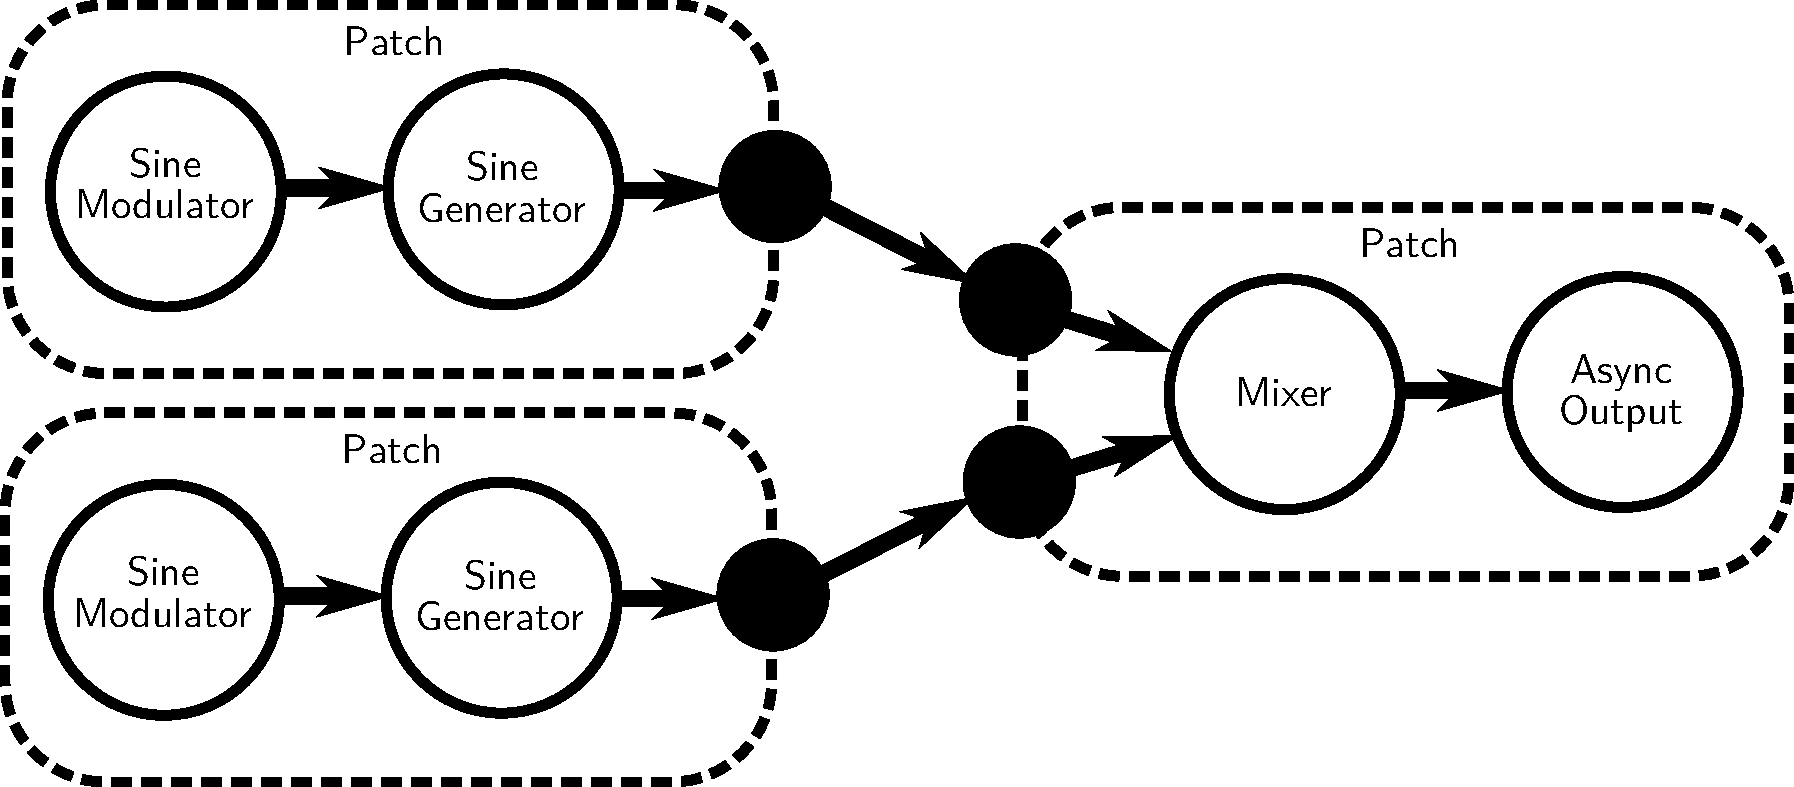
\includegraphics[width=\textwidth]{pic/graph-perf.pdf}
  \caption{Synthesis graph of the performance test program.}
  \label{fig:perfgraph}
\end{figure}

The program source code is in the
\type{src/test/examples/graph\_perf.cpp} file. The high amount of user
events stresses the synchronisation channels to find potential
implementation problems. It also has enough nodes to check if graph
traversal consumes too much time, and the presence of several patches
can show whether port forwarding is causing a significant overhead ---
it should not!

\subsubsection{Call graph profiling}

The Valgrind\footnote{\url{http://valgrind.org}}
\cite{nethercote07valgrind}\index{Valgrind} binary instrumentation
framework provides many tools for evaluating the performance and
correctness of programs by executing them in an instrumentated
environment --- a sort of machine simulator. In this section, we are
most interested in Callgrind \cite{weidendorfer04callgrind}, a
\index{Callgrind} profiler that generates an \index{call graph}
annotated call graph of a program's execution, indicating the amount
of time spent under each function and within the function itself. We
should expect that the time spent in the functions that we developed
in this chapter is little compared to that of doing the actual sound
processing and I/O. Because in section \ref{sec:sound-performance} we
already showed that our sound processing facilities are quite
efficient, that would evidence that the overall performance of the
system is acceptable.

\begin{mynote}[Other kinds of profilers]
  The Gperf\footnote{\url{http://www.gnu.org/software/gperf/}} tool
  does a similar job with a much more lightweight
  instrumentation. Heavy instrumentation can be a problem when running
  a program with real-time conditions like ours causing fake device
  \index{underrun}\emph{buffer underruns}, but a powerful enough
  machine often compensates. Indeed, \type{gperf} was not valid in our
  case because of its limitations with multithreading.

  Statistical profilers like
  Sysprof\footnote{\url{http://sysprof.com/}} and
  Oprofile\footnote{\url{http://oprofile.sourceforge.net/news/}} hook
  in the operating system and sample the current running process from
  time to time providing the least intrusive profiling. However, they
  provide much less accurate data and require long running times to
  yield good results. Actually, because of the barriers that the OS
  imposes in interrupting real-time threads, they are particularly
  unsuitable for our needs.

  We indeed tried all these tools and Valgrind provided the most
  accurate and useful results. The ease of use and polishment of the
  tools for visualising Callgrind's output also influenced our
  decision.
\end{mynote}

We ran the program with the command:
\begin{verbatim}
  $ valgrind --tool=callgrind ./example_graph_perf
\end{verbatim}

This generates a \type{callgrind.out.\$PID} file that can be
visualised and navigated with the \index{Kcachegrind}
Kcachegrind\footnote{\url{http://kcachegrind.sourceforge.net/}}
tool. It is usually hard to summarise a whole profille data in a
simple graph or table. Still, the resulting output supports our
thesis: the graph maintenance and thread communication system produce
negible overhead and most of the time is spent doing the sound
processing itself as we expected. Around a $18\%$ of the time was
spent in the \type{soft\_in\_buffers} because we apply the envelopes
in a sort of brute-force manner, but this is still little compared to
the $35\%$ that was spent generating sinusoids or the $38\%$ of time
that involved I/O with the sound card. Hence, it is not urgent to
optimise that and it would be relatively easy to do that anyway. The
Callgrind output file is included in the CD addendum such that the
skeptical reader can validate the output by herself. Figure
\ref{fig:callgrind-1} attempts to present the most significant parts
of the callgraph too.

\begin{figure}[h!]
  \centering
  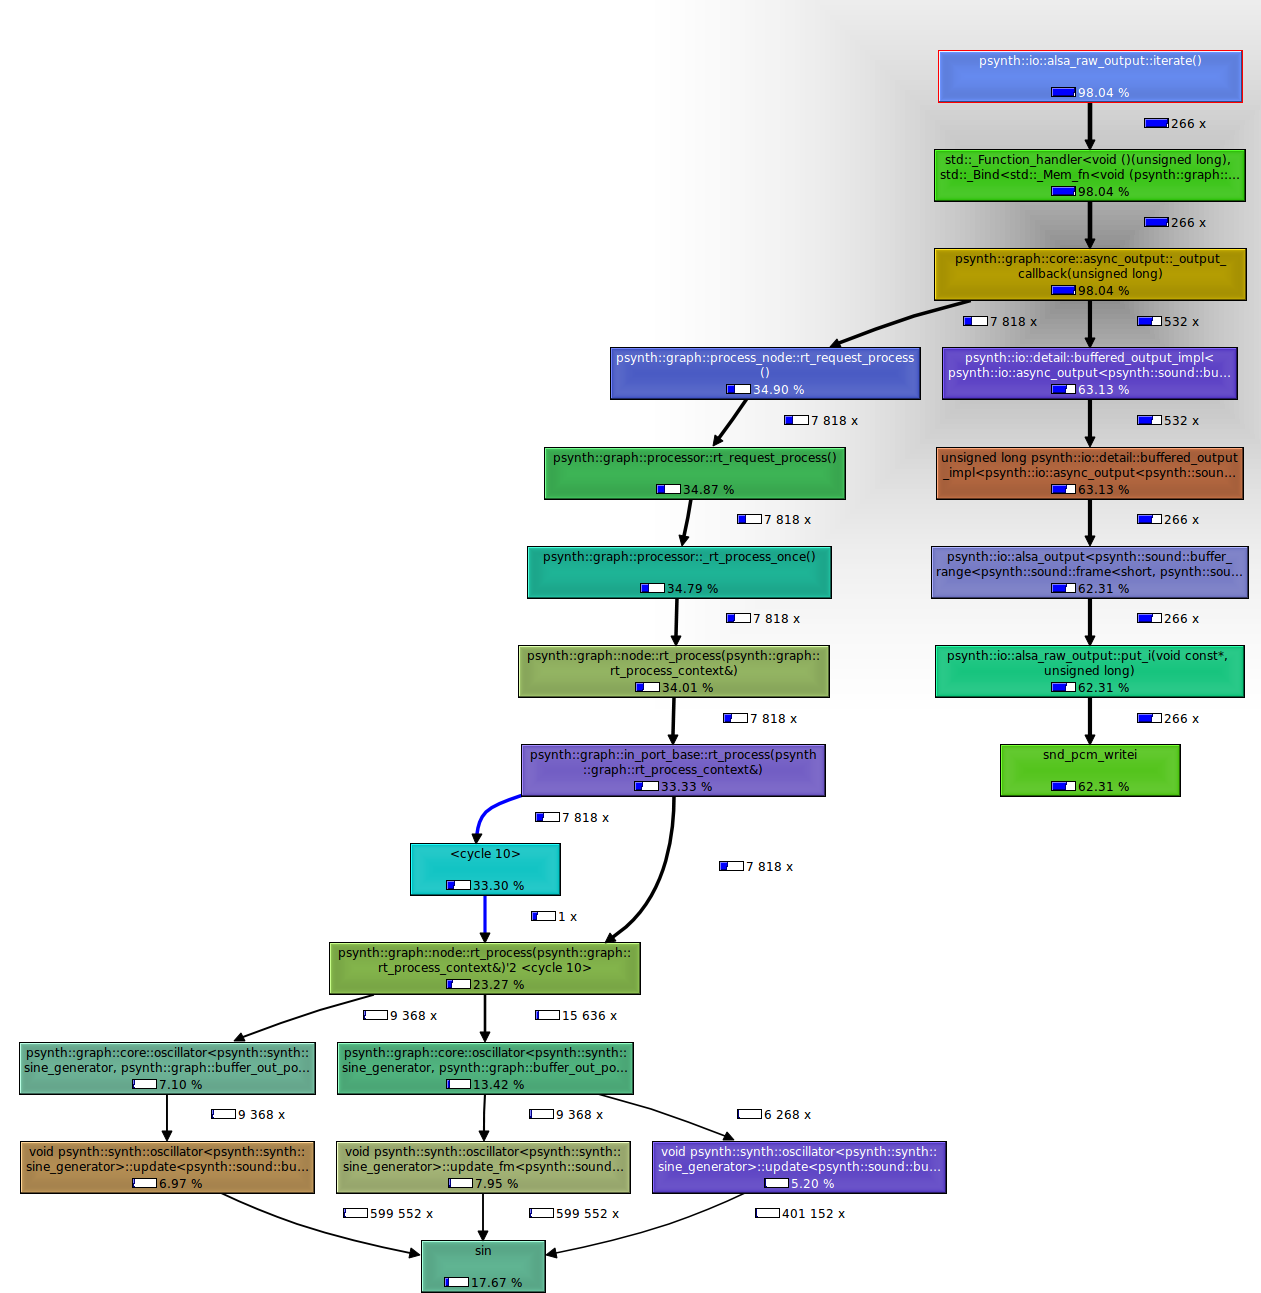
\includegraphics[width=\textwidth]{pic/callgrind1.png}
  \caption{Overview of the profiling call graph in the sound
    processing thread.}
  \label{fig:callgrind-1}
\end{figure}

\subsubsection{Validating real-time constraints satisfaction}

The \type{mutrace}\index{Mutrace} and \type{matrace}\index{Matrace}
tools profile the program to find much more specific patterns of
resource usage. The first one traces a program to find which locks are
used in a real-time thread, the number of contentions and the amount
of time spent both contending and withing the lock's critical
section. The later finds allocations and deallocations that happen
within a real-time thread. It uses a much more lightweight kind of
instrumentation that only relinks the application with wrapped
versions of \emph{pthreads} and \emph{libc} that allow the profiler to
collect the statistics. In order to run the program with these tools
we passed the following extra compile flags when building our program:
\begin{verbatim}
    -rdynamic -DPSYNTH_NO_LOG_RT_REQUEST
\end{verbatim}

The first option generates extra hooks for accessing the stack trace
at runtime allowing \type{mutrace} and \type{matrace} to provide
better information. The second disables logging a message into the
Psychosynth log system to inform the user that we succesfully got
real-time priority for the audio thread. When logging that message
several allocations are performed and critical sections are
entered. All this happens in the real-time thread, but it is done just
after it is launched and before we do anything useful, and thus it
only bloats the profiler output unnecessarily. 

Then, we run the program with parameter \verb|-r| to track real-time
threads and \verb|--all| to display information about all mutexes:
\begin{verbatim}
    $ mutrace -r --all ./example_graph_perf 2> mutrace-output
\end{verbatim}

\index{real-time}The most relevant bits of its output are illustrated
in note \ref{note:mutrace-output}. As we can see, none of the three
mutexes used in the real-time thread is ever contended. This is not
chance, repeated execution of the program yields the same results; it
is so because we always \type{try\_lock} from the real-time thread.

Note that the third mutex in the list --- mutex \#7 --- is the mutex
that synchronises calls to \type{rt\_request\_process} --- this can be
elicited from the \type{mutrace} output that was removed from this
summary. Because this mutex is locked exactly during each iteration of
the audio processing, two important performance facts can be derived
from its numbers:
\begin{itemize}
\item It was locked for a sum of $248.458 ms$ out of a total of
  $10065.873 ms$ running time. We can conclude from this that the
  sound processing took only a $2.465\%$ of the total running time,
  which insinuates that our synthesis graph can grow much larger.
\item It was locked $0.036 ms$ on average and a peak of $0.709
  ms$. The program was run with a block size of $64$ frames and a
  frame rate of $44100 hz$, giving a maximum latency of $1.45 ms$. This
  suggests that it is extremely unlikely for buffer underruns due to
  software overload.
\end{itemize}

However, it is rather intriguing the presence of inconsistent
mutexes\footnote{A mutex is said to be inconsistent when it remains
  locked after the owner thread terminates. The threading system
  unlocks it automatically, but it can signify of a software logic
  problem.}. The fact is, we are \emph{always} locking mutexes with
\type{unique\_lock}, so it is impossible for a mutex to remain
unlocked on scope exit. The further stack traces that \type{mutrace}
dump and that was removed from the fragment --- it can be checked in
the CD too --- suggest that it is an incompatibility between
\type{mutrace} and the sometimes subtle internal use of
\type{pthreads} in the C++0x threads API GCC implementation.

\begin{mynote}[\type{mutrace} output for the performance test program]
\scriptsize\label{mutrace-output}
\begin{verbatim}
...

mutrace: Showing 12 most contended mutexes:

 Mutex #   Locked  Changed  Cont. tot.Time[ms] avg.Time[ms] max.Time[ms]  Flags
       3     7435      205      0        1.820        0.000        0.011 M-R--.
       6     7028        3      0        1.862        0.000        0.020 M-R--.
       7     7025        0      0      248.458        0.035        0.709 M-R--.
      11     1065        0      0        4.427        0.004        0.099 M!---.
       2      429        0      0        0.294        0.001        0.022 M----.
       1       26        0      0        0.265        0.010        0.215 M----.
       0        8        0      0        1.093        0.137        1.046 M----.
       9        5        0      0        0.087        0.017        0.070 M!---.
       4        4        0      0        0.011        0.003        0.007 M----.
       8        4        0      0        0.007        0.002        0.004 M----.
      10        1        0      0        0.023        0.023        0.023 M----.
       5        1        0      0        0.000        0.000        0.000 M----.
                                                                         ||||||
                                                                         /|||||
          Object:                                   M = Mutex, W = RWLock /||||
           State:                               x = dead, ! = inconsistent /|||
             Use:                               R = used in realtime thread /||
      Mutex Type:               r = RECURSIVE, e = ERRRORCHECK, a = ADAPTIVE /|
  Mutex Protocol:                                    i = INHERIT, p = PROTECT /
     RWLock Kind: r = PREFER_READER, w = PREFER_WRITER, W = PREFER_WRITER_NONREC 

mutrace: Total runtime is 10065.873 ms.

...
\end{verbatim}
\end{mynote}

The twin tool \type{matrace} also provides relevant evidence on the
correctness of our program. We ran it typing:
\begin{verbatim}
    $ matrace ./example_graph_perf
\end{verbatim}

Note \ref{note:matrace-output} shows the most relevant parts of its
output. There are 5 allocations and 4 frees in the real-time thread
but they are not alarming at all. The stack traces removed from that
output summary reveal that they were performed just when the thread
started --- as a product of copying the \type{std::function} that the
\type{std::thread} constructor takes as argument --- and just when the
thread is about to be released --- performed by the \emph{pthreads}
internal data structures management.

\begin{mynote}[\type{matrace} output for the performance test program]
\label{note:matrace-output}\footnotesize
\begin{verbatim}
matrace: Total of 7381 allocations and 5747 frees in non-realtime 
threads in process lt-example_grap (pid 1617).

matrace: Total of 5 allocations and 4 frees in realtime threads.
\end{verbatim}
\end{mynote}

This section provided enough evidence that the performance of the
program is quite acceptable and that it meets our minimum guarantees
to control non-determinism and prevent clicks due to buffer underruns.

\subsection{Integration}
\label{sec:graph-integration}

Section \ref{sec:graphmvc} discussed how we chose not to integrate
this new module into the upper layers of the application yet. We shall
wait for the next iterations of the project --- which are out of the
scope of this master's thesis project --- to fully stabilise this API
and make the work of adapting the UI worth. However, we wrote some
example test programs that test interactions between modules further
than the unit tests. These programs are built in the \type{src/test}
directory and are:
\begin{description}
\item[example\_graph\_scale] Plays an $A$ note jumping among octaves
  among other events. It was one of the firsts test programs developed
  and helped to ensure that the control classes works properly.

\item[example\_graph\_patch] Plays some very strange sounds with
  patches nested up to several levels, with some patch ports that even
  change names during the playback and some other things. It helped to
  ensure that the interacting actors in the hierarchical patches
  system do work properly.

\item[example\_graph\_perf] This is the program that we described in
  the last section. It tries to simulate a rather dynamic and
  stochastic interaction with the system and ease profiling.

\item[example\_graph\_output] Tests outputting to two different
  proactive devices at the same time. Its synthesis network is very
  similar to that of the profiler program back in figure
  \ref{fig:perfgraph}. Apart from the output device that is already
  shown there, there is a second \emph{async output} connected on the
  output of the first synthesis patch. There are no random events;
  each generator-modulator has fixed constants with different out of
  phase frequencies. On one of the output devices one should listen to
  the sum of the two vibrating sinusoids, on the other just one of
  them. The test succeeded emitting at the same time on an on-board
  ``Intel 5 Series/3400'' sound card and an ``M-Audio Xponent DJ
  Controller'' USB integrated audio card.

\item[example\_graph\_soft] This program ensures that the ports with
  automatic reconnection softening actually do work properly. The
  network it executes is represented in figure
  \ref{fig:examplegraphsoft}. It generates three files,
  \type{graph-soft-N.wav}. 

  As illustrated in the figure, the program starts with a sine
  generator connected at the first of the two inputs of the greater
  patch --- these inputs do connetion softening. It generates 1024
  samples of a $880 hz$ sinusoid --- a pure $A_5$ in the ISO standard
  tuning \cite{pitchstd} --- and then it changes the connection to the
  second port that takes the signal into the patch. The audio output
  in the three files should then be something like what we described
  back in figure \ref{fig:soft-port-1} in section
  \ref{sec:modports}. We should expect the \type{graph-soft-1.wav}
  file to get something like the red line in that figure, a fade out
  after the disconnection. Then, the \type{graph-soft-3.wav} should
  show something like the green signal, a fade in when the generator
  is changed from one port to the other. Finally, the
  \type{graph-soft-2.wav} file should contain the sum of those two
  signals, similar to the dotted blue line in the plot --- it should
  remain as a stable pure tone without artifacts when the reconnection
  is made.

  The system passes this test as shown in figure
  \ref{fig:soft-audacity} where the output files are visualised with
  the Audacity program. When changing the connection, the signal is
  properly faded out and in avoiding any audible distortion.
\end{description}

\begin{figure}[h!]
  \centering
  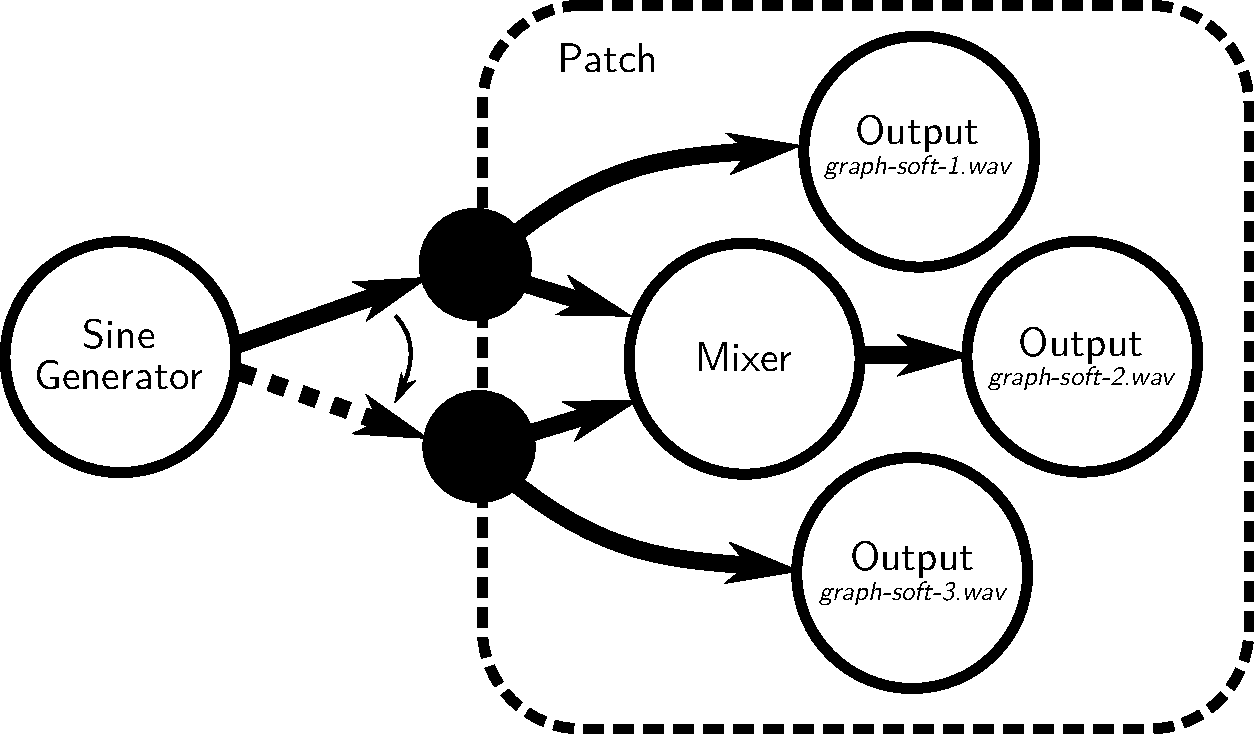
\includegraphics[width=\textwidth]{pic/graph-soft.pdf}
  \caption{Synthesis network of the reconnection softnening test
    program.}
  \label{fig:examplegraphsoft}
\end{figure}

\begin{figure}[h!]
  \centering
  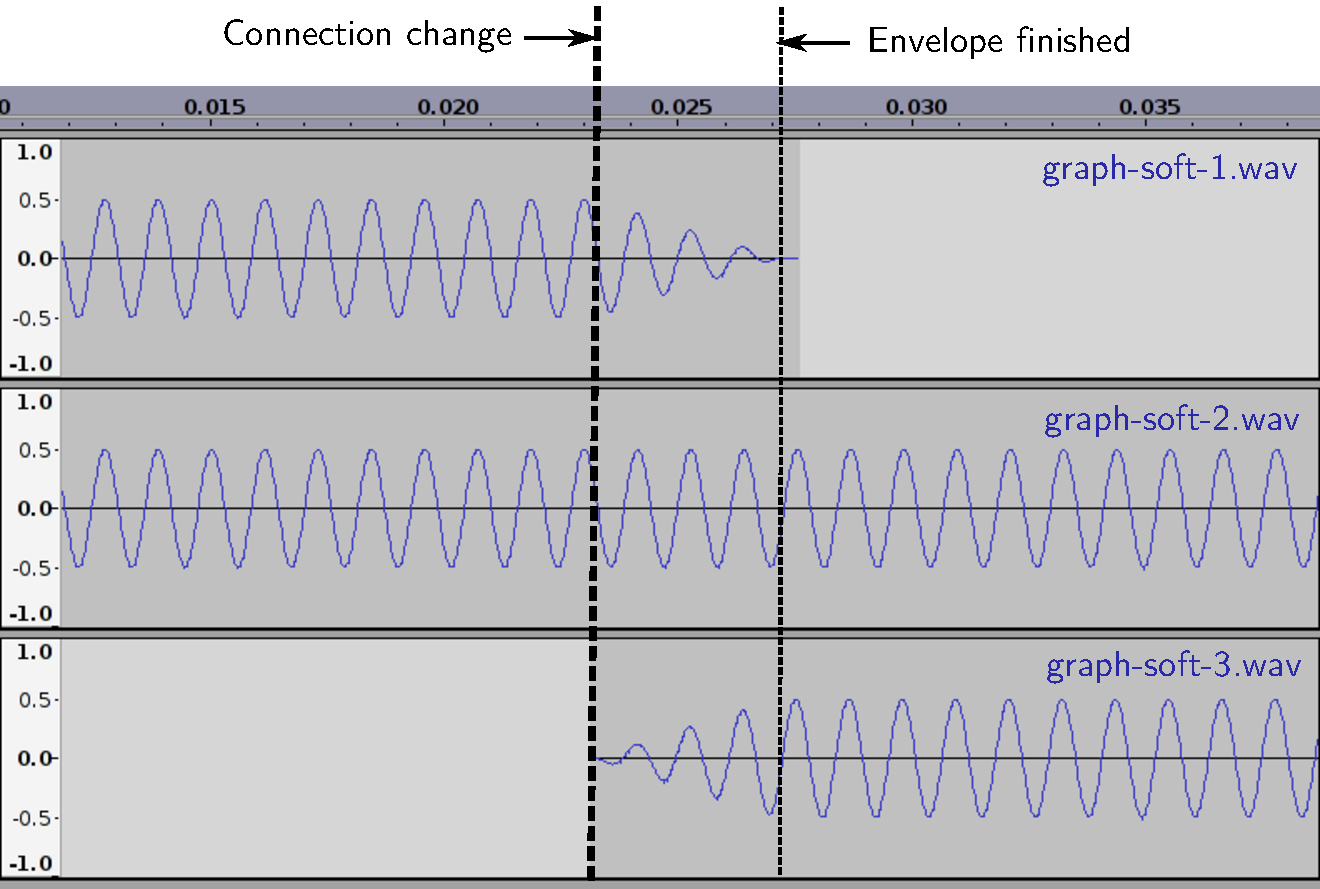
\includegraphics[width=\textwidth]{pic/sound-vis.pdf}
  \caption[The three output files in the reconnection softening test
  program.]{The three output files in the reconnection softening test
    program. The signals are, in this top-down order:
    \type{graph-soft-1.wav}, \type{graph-soft-2.wav} and
    \type{graph-soft-3.wav}}.
  \label{fig:soft-audacity}
\end{figure}

\todo{Hacer un release antes de enviar el proyecto a imprimir y poner
  aquí el changelog!!}

\section{Conclusion}

\index{multi-paradigm programming}In this second and last iteration of
this project we rewrote the whole modular synthesis engine of the
Psychosynth software in an attempt to solve the design problems of the
previous implementation and set up a solid base capable of being
extended with all the new features that are planned for the
future. Influenced by Van Roy's work \cite{roy04concepts},
multi-paradigm programming aided in writing an scalable design: (1)
generic programming and policy based design helped in avoiding
redundancy in the implementation, improves type safety thanks to
compile-time bound polymorphism and abstracts factors orthogonally,
(2) object-orientation provides dynamic reconfigurability and aided in
large-scale design and global system modularity, and (3) functional
programming allowed abstracting the control flow and helps in
controlling state and the exponential complexity growth when mixing
concurrency with stateful algorithms.

\subsection{Benefits and caveats}

There are few advancements in the new code that we should highlight:
\begin{enumerate}
\item Writing thread-safe code is usually quite challenging. Doing so
  in a real-time system is even harder. We abstracted the control flow
  using an event passing system that eases extending the program with new
  facilities that require inter-thread communication.

\item The new system is much more general and type safe in the
  processing. It is capable of processing signals of any kind in a
  type-safe manner --- whenever possible --- or throwing exceptions on
  type violations where dynamism is unavoidable.

\item The new design is much more decoupled, permitting the extension
  of the different components individually. For example, the fact that
  ports and controls are now objects instantiated by the concrete node
  type by itself, allows the development of new patterns of inter-node
  communication by deriving from these classes. A concrete example of
  this is the connection softening. That used to require a lot of work
  from the DSP implementer and it is now transparent and optional because
  an specific port object does the job. Another positive consequence
  of this new design is that implementing a plug-in system is now much
  more straightforward.
\end{enumerate}

There are some many other minor implementation improvements, like much
better error control, improved compilation process via the usage of
forward declarations and the absence of data races and dead locks that
the former implementation suffered.

This new implementation uses C++0x features and advanced C++
implementation techniques, so most of the reasoning in the conclusions
of the last chapter on the barrier that this might be for novel
developers applies up to some extent (section
\ref{sec:soundbenefits}). Still, in this layer, most of this
complexity is hidden in the implementation and does not get through
the public interface. Most of this complexity was caused by how
template programming errors can not be easily transcribed by
compilers, but most of the time, writing new DSP nodes or using the
external graph and processing interface relies on simpler and easier
to use object-oriented concepts that do not yield cryptic error
messages.

\subsection{Future work}

In spite of this positive general balance, there is much room for
improvement. There are many small improvements that have been
discussed already while describing the design and do no require
evaluating them here. Some other are either specially urgent or of a
broader scope and we should recapitulate them now.

\subsubsection{Lock-free heterogeneous deques}
\label{sec:improvehetero}

\index{flip (multiple buffering)}Our triple-buffered event deques
prevent locking from the RT thread as long as the ``flip'' can be done
conditionally. This means that if a event is being added to back deque
from the user thread just when the RT thread is attempting the flip,
the flip might be skipped and events in the back buffer would need to
wait for the next control iteration. Inserting user event happens
sparely enough for this pattern to work, as our experiments
show. However, this prevents implementing some other techniques that
are more demanding --- we assumed that events are caused by user
interaction most of the time, but it can be interesting for some
applications to generate huge amounts of events programatically.

\index{lock-free algorithm}\index{heterogeneous deque}If our
heterogeneous deques where lock-free --- i.e. they support one reader
and one writer at the same time in different threads --- the flip
would need no locking at all and it could be always achieved
regardless of what the user thread is doing. We already cited Valois'
work on lock-free data-structures \cite{valois96lockfree,
  michael95correction}. Our heterogeneous deques unique nature do not
have a direct mapping to any of the data structures in the
bibliography, but some authors provided design techniques to elicit
our own lock-free datastructures. Harris improvements for node-based
structures can be of great help \cite{harris01pragmatic}. There is
plenty of other bibiography we can refer to\footnote{We do not want to
  flood this document with references to lock-free algorithms. A good
  compilation has already been made by Ross Bencina:
  \url{http://www.rossbencina.com/code/lockfree}}.

\subsubsection{``Futures'' API for the asynchronous events}

We described how the ``asynchronous operation'' thread can be used by
the RT thread to delegate costly not urgent operations --- like
allocating heap memory or doing I/O. Very often, that requires
returning a result back --- for example, the pointer to the allocated
memory. It is not hard to do so, but it requires adding extra
redundant code. The C++0x standard includes the notion of
\emph{future}, a value that is computed, potentially, in a separate
thread, leading to more declarative concurrency
\cite{howard06mt}. Still, these are not usable in a real-time context,
because computing a future requires creating a dynamic functor,
launching threads, allocating memory and so on. However, its API can
be emulated on top of our thread communication infrastructure,
simplifying this common pattern of requesting some computation in the
``async thread'' and using its result later. In some way, this is just
extending the event system with a notion of ``event with a return
value''.

\subsubsection{Compiling static networks}

In this iteration we concentrated on the dynamic features of our
synthesis system. This often trades-off performance. This is ok as
long as enabling live music is our most important objective. However,
getting some nice sounds often requires sitting down in the studio and
doing \emph{sound design}\index{sound design} and implementing complex
mathematical functions by assembling lots of low-level modules into a
patch. These patches are too low-level to be manipulated in a live
performance and thus dynamism can be exchanged for a performance gain,
needed to handle such big amounts of small nodes. Some software
implementing these kind of features, like Reaktor's ``Core-Cell
Modules'', traduce the network into a compiled form optimised for fast
execution. This can be a very interesting development to broaden the
scope of the project. However, it requires a lot of effort and is not
very urgent --- sound design and DSP programming can already be done
either directly in C++, or in other synthesis systems and then plugged
in when the plug-in system is ready --- so we propose it as later
future work.

%%% Local Variables: 
%%% mode: latex
%%% TeX-master: "00-main"
%%% End: 
